\documentclass{article}
\usepackage{setspace}
\usepackage[explicit]{titlesec}
\usepackage{forest}
\usepackage{hyperref}
\usepackage{graphicx}
\usepackage{listings}
% Used for creating clean tables within app
\usepackage{booktabs}
% Used for creating check marks in app, amongst others
\usepackage{amssymb}
% Used for creating gray color background boxes
\usepackage[breakable, theorems, skins]{tcolorbox}
% dirtytalk is used for quotation marks using \say{}
\usepackage{dirtytalk}
\DeclareRobustCommand{\mybox}[2][gray!20]{%
\begin{tcolorbox}[   %% Adjust the following parameters at will.
        breakable,
        left=0pt,
        right=0pt,
        top=0pt,
        bottom=0pt,
        colback=#1,
        colframe=#1,
        width=\dimexpr\textwidth\relax,
        enlarge left by=0mm,
        boxsep=5pt,
        arc=0pt,outer arc=0pt,
        ]
        #2
\end{tcolorbox}
}

\definecolor{folderbg}{RGB}{124,166,198}
\definecolor{folderborder}{RGB}{110,144,169}

\def\Size{4pt}
% Drawing for folder directories across app
\tikzset{
  folder/.pic={
    \filldraw[draw=folderborder,top color=folderbg!50,bottom color=folderbg]
      (-1.05*\Size,0.2\Size+5pt) rectangle ++(.75*\Size,-0.2\Size-5pt);
    \filldraw[draw=folderborder,top color=folderbg!50,bottom color=folderbg]
      (-1.15*\Size,-\Size) rectangle (1.15*\Size,\Size);
  }
}
\definecolor{lightgray}{rgb}{.9,.9,.9}
\definecolor{darkgray}{rgb}{.4,.4,.4}
\definecolor{purple}{rgb}{0.65, 0.12, 0.82}
\definecolor{black}{rgb}{0, 0, 0}

\lstdefinelanguage{JavaScript}{
  keywords={typeof, new, true, false, catch, function, return, null, catch, switch, var, if, in, while, do, else, case, break},
  keywordstyle=\color{blue}\bfseries,
  ndkeywords={class, export, boolean, throw, implements, import, this},
  ndkeywordstyle=\color{darkgray}\bfseries,
  identifierstyle=\color{black},
  sensitive=false,
  comment=[l]{//},
  morecomment=[s]{/*}{*/},
  commentstyle=\color{purple}\ttfamily,
  stringstyle=\color{red}\ttfamily,
  morestring=[b]',
  morestring=[b]"
}

\lstset{
   language=JavaScript,
   backgroundcolor=\color{lightgray},
   extendedchars=true,
   basicstyle=\footnotesize\ttfamily,
   showstringspaces=false,
   showspaces=false,
   numbers=left,
   numberstyle=\footnotesize,
   numbersep=9pt,
   tabsize=2,
   breaklines=true,
   showtabs=false,
   captionpos=b
}

\forestset{
  default preamble={
    for tree={
      font=\ttfamily,
      grow'=0,
      child anchor=west,
      parent anchor=south,
      anchor=west,
      calign=first,
      inner xsep=7pt,
      edge path={
        \noexpand\path [draw, \forestoption{edge}]
        (!u.south west) +(7.5pt,0) |- (.child anchor) pic {folder} \forestoption{edge label};
      },
      % style for your file node
      file/.style={edge path={\noexpand\path [draw, \forestoption{edge}]
        (!u.south west) +(7.5pt,0) |- (.child anchor) \forestoption{edge label};},
        inner xsep=2pt,font=\small\ttfamily
                   },
      before typesetting nodes={
        if n=1
          {insert before={[,phantom]}}
          {}
      },
      fit=band,
      before computing xy={l=15pt},
    }
  }
}


\title{Angular - The Full Gamut}
\author{Charlie Greenman}
\renewcommand{\familydefault}{\sfdefault}
\begin{document}

\setstretch{1.5}
\tableofcontents
\maketitle{}
\section{Introduction}

The current landscape of UI development is in a very interesting place, for many
reasons. For starters, the mere capacity of web to do many tasks previously
unavailable(Add examples here), is growing by the year. In addition, frameworks
which allow for scalability, DRY development, and consistency is ever going. In
your average web application, it generally includes type checking, unit testing,
integration testing, as well as state management, and observables/effects. These
are all things that 3 years ago were not common place in the enterprise, and it
is only becoming a greater landscape as time goes on.

Angular in my opinion, having worked with other frameworks such as Elm, Vue,
React, and Cycle, is in a very unique place. I will admit, there are many
reasons as to why other to use other front end frameworks(, or if you prefer to
not call them frameworks, I understand that as well). For instance, Vue, is very
simple to use. React, is always on the cusp of cutting edge. Reason in
particular as of this writing is simply incredible. Cycle, in it's approach
towards functional programming, is refreshing. However, Angular specializes in
consistency, therefore productivity, as well as safety.

It does not surprise me that the most robust command line, by a long shot, is
with Angular. Everything, from how to style a component, folder structure,
routing, observables, state management, type checking, is agreed upon by the
entire Angular community. It is a very safe bet when building out an enterprise
application. It makes architectural decisions very easy, and it does have the
ability to layer on newer technologies, if need be, albeit harder than some
frameworks such as React. It does not surprise me, that the first full gamet
book will be written on Angular. It towers over the rest in consistency, and
that deserves a head nod.

The issue with many technical books, is that as a reader I will walk away from
it feeling like I scratched the surface. That is, I am not confident I have
covered the full gamut of that topic. So that if I plan on building it myself,
I still have to do research on my own. In addition, when I do plan on building
an app, I do not have an example app to work against. Essentially making the
book useless. Like seriously, it has me wondering the benefit of many of the
technical books I've reading lately!

As of now, it pretty much helps as discovery, and for maintaining new material.
However, learning it does not help. This book on the other hand will help you,
really one of the first of it's kind and sort of revolutionary. By offering a
QR code, with the latest commit, linked to a stackblitz, you will simaltaneously
be able to follow along while reading the book, seamlessly. In addition, when
you have read the entire book, and need to reference bits here, and there,
you can look at a specific commit for a certain part of the book, and remind
yourself how to do it once again.

In this the full gamut series, we will build a sample application. The
application will be a pixel illustrator. The ability to draw a pixel on an
artboard, and plot the coordinates on the left side. In addition, the ability to
change colors on the right side.

The intent of the book, is that it will be built in the most cuting edge
capacity. The reader should be walking away knowing, that what they have learnt
from this book is best practices, as well the Full Gamut of Angular. Being
confident, that they are aware of the full scope of the Angular ecosystem at
this time.

In addition, conventions will be casually sprinkled from time to time.
Conventions are on wide spectrum of impact. Some conventions beckon being
chosen, while others are chosen without the thought of doing so. From an
architectural perspective, they are equally as important, because choosing them
ahead of time, will save days of unneccesary re-factoring. This book as a result
will also consider conventions as part of it's architecture, and will put them
in a blue box.

In addition, this book acknowledges that there are three parts to learning:
\begin{enumerate}
  \item Discovery
  \item Maintaining
  \item Learning
\end{enumerate}

Some parts of this book are discovery, and some parts are learning. This are
parts that every book has, but this one would like to also add maintenance to
the mix. As we build out our app throughout this book, we will also repeat steps
when possible, that we have already learnt.

Part of the value of this book as well, is if this is something that you would
like to implement, the time can be minimized by using the content mentioned
in this book.

In addition, for the core part of this book. I tried, to make the core
documenation as similar to that, that can me found in the documenation, to make
it as least confusing as possible for the reader.

Some might consider this book opinion. However, after working at 5 different
companies, I can say with confidence that they all could have used the same
architecture, and component library. That is, if you a web application, that
is data heavy, trying to allow user to interact with said data, creating,
removing, updating, and deleting, this architecture will work for you. It is
therefore my opinion that this is the singular best architecture for Angular,
and I feel 100\% comfortable calling it the Definitive Guide.

Also, the idea of a good architecture, isn't neccesarily so that it goes through
everything. The idea of good architecture, is so that if something new comes up,
you will be able to have to drastically change your codebase.

This book is going to be app agnostic. However, it is going to work against the
app in order to show how technology should be integrated in real time. In
addition, there is going to be commits made in the repo alongside the book,
so that it can give a better idea of how this architecture will work in real
time.

Each section is meant to be looked through throughly before one goes ahead and
one actually does actual wokr on them. For instance, for the section on state,
it goes through the architecture for all sections on the ngrx/store. Only once
it does so, will it go through the folder/file architecture for state.


\chapter{ Building our Application }

In order to go through the full gamut of Angular, we are going to focus on as
lightweight of an application as possible. In order to go through entire Angular
architecture, we obviously do not want to over due it, nor do too little. It
goes without saying, that your classic todo app, will not suffice. Instead the
following is the application that we will be building.

We are going to call it a pixel to coordinate illustrator. The idea behind the
app, is that we should have a canvas, paint a pixel on that canvas. We then have
a coordinate, that will appear based on where pixels are currently located.

In our application we have:
\begin{enumerate}
  \item Form
    \begin{enumerate}
      \item Pixel Size
      \item Number of Rows
      \item Number of Columns
    \end{enumerate}
  \item Color Picker
    \begin{enumerate}
      \item Background Color Picker
      \item Pixel Color Picker
    \end{enumerate}
  \item Pixel Canvas
    \begin{enumerate}
      \item Pixel Grid
      \item Ability to Remove Pixel
      \item Ability to Add Pixel
      \item Ability to Change Pixel Color
    \end{enumerate}
  \item Coordinate Viewer
    \begin{enumerate}
      \item Show x Coordinate
      \item Show y Coordinate
      \item Show Pixel Size
      \item Show Pixel Color
    \end{enumerate}
\end{enumerate}

Application will be made responsive. Without further ado, let's begin our
applcation.


\section{ Versioning }

\subsection { Git }
It goes without saying that you should be using Git. Unless you have an
incredibly huge diffing tree in your repo, which is most of us, then you should
be using Git.

\subsection { Integration with JIRA }
In any JIRA ticket, if one has the proper webhooks setup with Github, or if one
is using BitBucket, then it will automatically hook up the commit into the
ticket. All that is neccesary, is for the the commit message to include the
ticket name. (Screenshot for example should go here).

\subsection { Analyzing a Git Branch }
In any git environment, the name of the git branch is important for the
following reasons:

\begin{enumerate}
  \item It can inform the developer about the type of branch
    \begin{enumerate}
      \item feature
      \item hotfix
      \item bugfix
      \item refactor
      \item cleanup
    \end{enumerate}
  \item It can inform the developer of ticket being worked on
  \item It can inform the developer of abstract of ticket.
\end{enumerate}

In addition, as we have mentioned above, it will be particularly advantageous to
having the branch name, when it comes to integrating with JIRA.

\subsection { Branching Name Convention }
Let's imagine our project is called PIXE. We have a ticket called PIXE-113,
which is responsible for adding a pixel color picker to our Pixel Illustrator
app. We would create our branch as following:

\begin{verbatim}
  feature/PIXE-113-details-and-actions
\end{verbatim}

\begin{itemize}
  \item feature is name of issue type all lowercase followed by forward slash
  \item PIXE-113 is name of ticket in all caps, followed by dash
  \item details-and-actions is abstract of ticket
\end{itemize} \marginpar{Todo: Create a graphic for this one}

\subsection { Git Client }
When it comes to using an IDE, I strongly believe that every team member should
have the freedom to use whatever they want. It is very important, in general,
that all team members feel free to use whatever they want. In this same vein
they should feel comfortable in using a client if they would like. I personally
prefer using the terminal.

\subsection { Fork and Pull Workflow }
It is reccomended to use a fork and pull workflow. There are a number of
benefits to adopting such a workflow. Most importantly, however, is the
realization, that setting up a workflow the sooner the better is for a project.
In addition, the realization, that it is a one time setup.

\subsubsection { Setting up a Fork and Pull Workflow with Github }
Similar to how in this book we reccomend the usage of particular architecture,
we also reccomend specific platforms to use. We will run through this workflow
with Github, however, it is very possible with any other client.

Click on the button which says fork: (Include image for fork here).
Then go ahead


\subsection { Squash and Merge }
Github, is our preferred client. It gives the option to squash and merge a
particular commit. Squashing your commits should be your preferred way of doing
commits. It allows for a clean git history. By having a clean git history, one
can create a very clean version log, which specifies which features were built
in the latest version.

\maketitle{}
\section{ Technical Design Notes }

When creating a ticket, it is important that technical design notes be written
as a part of actual JIRA ticket.

\subsection{ What are Technical Design Notes? }
Technical Design Notes are a way to abstract the decisions one will make
towards architecting an app.

\subsection{ Benefits of Creating Technical Design Notes }
It allows the app to be thought through before app is built. Saving time on
re-factoring code, ensure code quality, and retain confidence that tickets will
be done the way they should be done.

\subsection{ When to Create Technical Design Notes }
Technical Design Notes can be cumbersome, and writing them does not make sense
in all instances. In one of two situations, technical design notes should be
created, when one, or more of the following is true:

\begin{enumerate}
  \item When Unit Testing is involved. For instance, let's say we have a
  filtering component, and we need to test what will happen if a user inputs a
  word with a space in it, or with a uppercase character.
  \item When strategy architecture is involved. For instance, we need to create
  a strategy for routing, or how we will end up pulling in data. Sometimes, it
  is something which will be an unknown, and saying this is what I am trying to
  figure out, and it is a unknown is more than perfect.
\end{enumerate}

\subsection{ What Goes into Technical Design Notes }
It should mention at a very high level, what should go into the component. For
instance, if I am building a filter, it should mention:
\begin{enumerate}
  \item That I plan on using ngrx/store in order to store filters.
    \begin{enumerate}
      \item Specifically as strings
    \end{enumerate}
  \item Will be using <md-input> material design component for filters.
  \item Will be writing integration test for filters individually, and how they
  will interact with each other.
  \item Will be creating filters for the following test scenarios.
    \begin{enumerate}
      \item Camel case
      \item Space in filter
      \item Pure text
      \item Dates
    \end{enumerate}
\end{enumerate}


\chapter{ Acceptance Criteria }
Acceptance Criteria should generally not be in the court of the software
engineer. However, as is quite common in software engineering, product will
need a bit of prodding from engineering, in order to discuss what it is that
they are looking for.

\section{ Real Quick - What are Acceptance Criteria? }
They are the conditions that a software product must satisfy to be accepted by
a user, customer, or in the case of system level functionality, the consuming
system.

\section{ Ideal Syntax for Acceptance Criteria? }
After being in a number of settings, the ideal way to create acceptance criteria
is to use Cucumber/Gherkin syntax.

\section{ What Gherkin Syntax? }
Gherkin is a syntax which supports BDD. It is aimed at making executable
specifications written in plain language\footnote{We will get to how we will
integrate this with our QA efforts in a moment}:
\begin{verbatim}
  Scenario: eat 5 out of 12
  Given there are 12 cucumbers
  When I eat 5 cucumbers
  Then I should have 7 cucumbers
\end{verbatim}

\section{ Why is it important that we use Gherkin Syntax? }
Gherkin syntax is designed to be succint, and easily understandable which it is.
In addition, it is a syntax that the entire company can rally around, being that
it will be used by Automation Engineers as well\footnote{Surpise! They will be
using Gherkin as well, unless you knew that one already. In which case it is
not a suprise.}. It is also in my experience, the only way to convince product
to write acceptance criteria that actually stays the same from ticket from
ticket, but don't tell them I said that!

\section{ Sample Ticket Creation for Choose Size Form. }
\begin{verbatim}
Scenario: When Using the Choose Size picker
  Given I enter pixel size
  Given I enter column size
  Given I enter row size
  When I  click on the Create Pixel Grid button
  Then I should see grid created
\end{verbatim}

Note that this is the ticket for creating a component for the choose size picker.
However, we still do now know what the design will look. This we leave for the
next chapter.


\chapter{ Ticket Creation - Component Design }
We have discussed the two initial steps with regards to creating a ticket.
Technical Design Notes, and acceptance criteria. The third and final step
with regards to any good ticket is design. The chapter regarding talking to
UI/UX is not here, but you should be using JIRA as your ticketing system.

Within a JIRA setting, two things should happen so you have a clear idea of
how a component should be designed within a PWA setting:

\begin{enumerate}
  \item Description
  \item Invision Link within JIRA
\end{enumerate}

\section{ Component Design Quirk }

When creating a ticket in a PWA environment, there is a need to create a specify
the specific functionality around mobile, and desktop. Many times, the
functionality is not the same. In addition, while we develop from a mobile first
perpective, it is not the case for business and product. For engineers, there
is an understanding that whatever is not used for mobile, is used for desktop.
This is not the case for business. They look at the two as two separate
entities.

In addition, understandably for design, they also look at mobile and desktop as
two different entities.

It is therefore reccomended that you will have to create two separate tickets.

\mybox{
\section{ Development Corner }
Having two tickets for mobile and development will cause conflict with regards
to pull requests. In order to solve this concern, make git commit's against
the web ticket. In addition, in your JIRA ticket, make mobile dependent on the
web ticket.
}

\maketitle{}
\section{ Angular CLI }

In any Angular setting the Angular CLI(Command Line Interface) is going to be
a good friend. The following are things which you are able to do, in the Angular
CLI:

\begin{enumerate}
  \item Create an application out of the box
  \item Generate a module
  \item Generate a component
  \item Generate a route
  \item Generate a service
  \item Serve application
  \item Test application
  \item Lint application
\end{enumerate}

\maketitle{}
\section{Introducing Nrwl Nx}

\subsection{Arguably–The Greatest Strength of Angular}

Arguably one of the greatest strengths of the Angular(2+) ecosystem is
consistency(a point we've discussed before). As a result, Angular has the most
advanced Front End Framework CLI.

\subsection{Angular CLI Shortcoming with Regards to State Management}

However, the Angular CLI does not deal with state management. State management
in Angular2, for the most part should be done using NGRX. State management in
it's self, however, can be unwieldy. For every new reducer, a new constant file,
as well as action, effect, and proper unit testing files are needed.
In addition, the Angular Framework is not built around state management. It is
easy for it to fall through the cracks, and for an app to be done without it in
the first place. Introducing the Nrwl nx CLI.

\subsection{NX CLI}
NX is built by a team called Nrwl. They are perhaps thought leaders in the
Angular space, as they well should be, being that a large part of them came
from the core Angular team. They decided to build a cli around state management.
However, using their cli comes the following pre-conditions, include the NX
Workspace.

\subsection{Introducing the NX Workspace}
One of the things that the Nrwk team really tries to push, that isn't mainstream
yet, is the concept of a workspace. Perhaps you will remember an article
floating around a while back, about
\href{https://cacm.acm.org/magazines/2016/7/204032-why-google-stores-billions-of-lines-of-code-in-a-single-repository/fulltext}
{Google's Mono Repo}. [Worth noting, this idea
has been popularized at
\href{https://code.facebook.com/posts/218678814984400/scaling-mercurial-at-facebook/}{Facebook}
as well]. The idea is that there is a singular repository for everything.
The benefits of such are
(\href{https://nrwl.io/nx/why-a-workspace}{Taken from Nrwl site}):

\begin{enumerate}
  \item Unified versioning
    \begin{enumerate}
      \item Everything at that current commit works together
      \item A label or branch can capture the same
    \end{enumerate}
  \item Promotes code sharing and reuse
    \begin{enumerate}
      \item Easy to split code into lib modules
      \item Easy to consume implement that code and the latest changes to it
    \end{enumerate}
  \item Easier dependency management
    \begin{enumerate}
      \item One node\_modules for all code
      \item One build setup (like the AngularCLI)
    \end{enumerate}
  \item Refactoring benefits
    \begin{enumerate}
      \item Code editors and IDEs are "workspace" aware
      \item Can have a single commit for a refactor that spans applications in the domain
    \end{enumerate}
  \item Consistent developer experience
    \begin{enumerate}
      \item Ensures all necessary dependent code is available
    \end{enumerate}
\end{enumerate}

Some of the biggest disadvantages include:
\begin{enumerate}
  \item Taking time to limit access to part of workspace.
  \item One upgrade in a lib, changes all areas.
  \item Make it overkill to work on a small feature.
\end{enumerate}

\maketitle{}
\section{ Nx Lib Conventions }

\section{ Why is an NX Workspace different than an NPM Repo }
One of the difficult things when starting with an Nx workspace for the first
time, is comparing it to an NPM repo. One may ask, why is it different than an
actual NPM repo?

\begin{enumerate}
  \item All code in the lib can be modified by any one person in the
  ogranization, as opposed to an NPM repo. It is therefore cheaper, and faster.
  \item There is no need to upgrade dependencies. Editing and updating a lib,
  will automatically affect all apps.
  \item It is cheaper to create a lib, as opposed to creating a new NPM package.
  No need to set up a CI/CD, or otherwise.
\end{enumerate}


\section{ Lib File Structure }

When working in a monospace repo, file archticture is very important, as
different parts of an application tend to be abstracted. First let's outline
the different potential parts of an Angular application.


\begin{forest}
  [libs
    [common
      [animations
      ]
      [assets
      ]
      [core
       [auth]
       [guards]
       [pipes]
       [validators]
      ]
      [models
      ]
      [testing
      ]
      [ui
      ]
      [utils
      ]
      [styles
      ]
      [vendor
      ]
    ]
  ]
\end{forest}

\subsection{ Lib File Structure in Detail }

\subsubsection{Animations}
Animations are where any common animations might go. Things such as ripple
effects, ghost elements, etc. Animations are really a whole different science
when it comes to development, and therefore makes sense for them to have their
own folder.

\subsubsection{ Assets }
This is where commonly re-used assets, such as icons, or logos are used.

\subsubsection{ Core }
Any piece of functionality that is re-used the app is used here.

\subsubsection{ Models }
This is where interfaces used across the app are used. This will simply type
annotations across the app. In addition, when using a place to reference the
full capacity of data requests within app, this model will be a life saver.

\subsubsection{ Testing }
All data mocks that are common, can go here as well. Data tends to be re-used
many different times within different parts of apps. So ideally, all mocks
should go here.

\subsubsection{ UI }
All presententational components go here. Some examples of might go into an
example app is a header, footer, loading spinner, or charts.

\subsubsection{ Utils }
Shared services used across different apps. For instance, dates.

\subsubsection{ Styles }
Any shared styles used across app, for instance spacing, media queries etc.

\subsubsection{ Vendor }
The vendor folder is used to customized 3rd party libraries. Some libraries
customized might include Angular Materal.


\section{ Lib File Structure }

When working in a monospace repo, file archticture is very important, as
different parts of an application tend to be abstracted. First let's outline
the different potential parts of an Angular application.


\begin{forest}
  [libs
    [common
      [animations
      ]
      [assets
      ]
      [core
       [auth]
       [guards]
       [pipes]
       [validators]
      ]
      [models
      ]
      [testing
      ]
      [ui
      ]
      [utils
      ]
      [styles
      ]
      [vendor
      ]
    ]
  ]
\end{forest}

\subsection{ Lib File Structure in Detail }

\subsubsection{Animations}
Animations are where any common animations might go. Things such as ripple
effects, ghost elements, etc. Animations are really a whole different science
when it comes to development, and therefore makes sense for them to have their
own folder.

\subsubsection{ Assets }
This is where commonly re-used assets, such as icons, or logos are used.

\subsubsection{ Core }
Any piece of functionality that is re-used the app is used here.

\subsubsection{ Models }
This is where interfaces used across the app are used. This will simply type
annotations across the app. In addition, when using a place to reference the
full capacity of data requests within app, this model will be a life saver.

\subsubsection{ Testing }
All data mocks that are common, can go here as well. Data tends to be re-used
many different times within different parts of apps. So ideally, all mocks
should go here.

\subsubsection{ UI }
All presententational components go here. Some examples of might go into an
example app is a header, footer, loading spinner, or charts.

\subsubsection{ Utils }
Shared services used across different apps. For instance, dates.

\subsubsection{ Styles }
Any shared styles used across app, for instance spacing, media queries etc.

\subsubsection{ Vendor }
The vendor folder is used to customized 3rd party libraries. Some libraries
customized might include Angular Materal.


\chapter{ Tsconfig }

\section{ What is the Tsconfig? }
The tsconfig file corresponds to the configuration of the Typescript compiler.

\section{ What the Default Tsconfig Looks Like. }
Angular CLI will generate a tsconfig out the box:
\begin{lstlisting}
  {
    "compileOnSave": false,
    "compilerOptions": {
      "sourceMap": true,
      "declaration": false,
      "moduleResolution": "node",
      "emitDecoratorMetadata": true,
      "experimentalDecorators": true,
      "target": "es5",
      "typeRoots": [
        "node_modules/@types"
      ],
      "lib": [
        "es2017",
        "esnext.asynciterable",
        "dom"
      ],
      "baseUrl": ".",
      "paths": {
        "@angularPixelIllustrator/*": [
          "libs/*"
        ]
      }
    },
    "exclude": [
      "node_modules",
      "tmp"
    ]
  }
\end{lstlisting}


\section{ Notable Mention }

\subsection{ sourceMap }
Source map true, will help debugging while using the console in the browser.
However, when debugging unit tests, it will cause somewhat of an issue.
Switching this to false at times can be helpful. Alternatively, one can hijack
the npm script for npm run test using.
\begin{verbatim}
  --source-maps=false
\end{verbatim}

\section{ Using paths }
Being that we are using a mono repo, if we were to pull components from within
the lib folder, we would have to use a very long relative path. However,
tsconfig has an option to specify a specific path. If you look above, in the
tsconfig, you will notice that there is a defauly path for libs, called the
angularPixelIllustrator.

In most cases the default name will suffice. However, in our scenario, let's
shorten the lib path to just ill.

\begin{lstlisting}
+      "@ill/*": [
-      "@angularPixelIllustrator/*": [
\end{lstlisting}

Now, whenever we would like to import a module/component from the lib folder
from within our app all we have to do is the following\marginpar{We are using
a barrel file, will get to that in a bit}:
\begin{lstlisting}
import {module} from '@ill/color-picker';
\end{lstlisting}

\maketitle{}
\section{ Barrel File }

\subsection{ What is a Barrel File? }

A barrel File is a way to rollup exports from several modules into a signle
convenience module. The barrel itself is a module file that re-exports selected
exports of other modules.
\\
\\
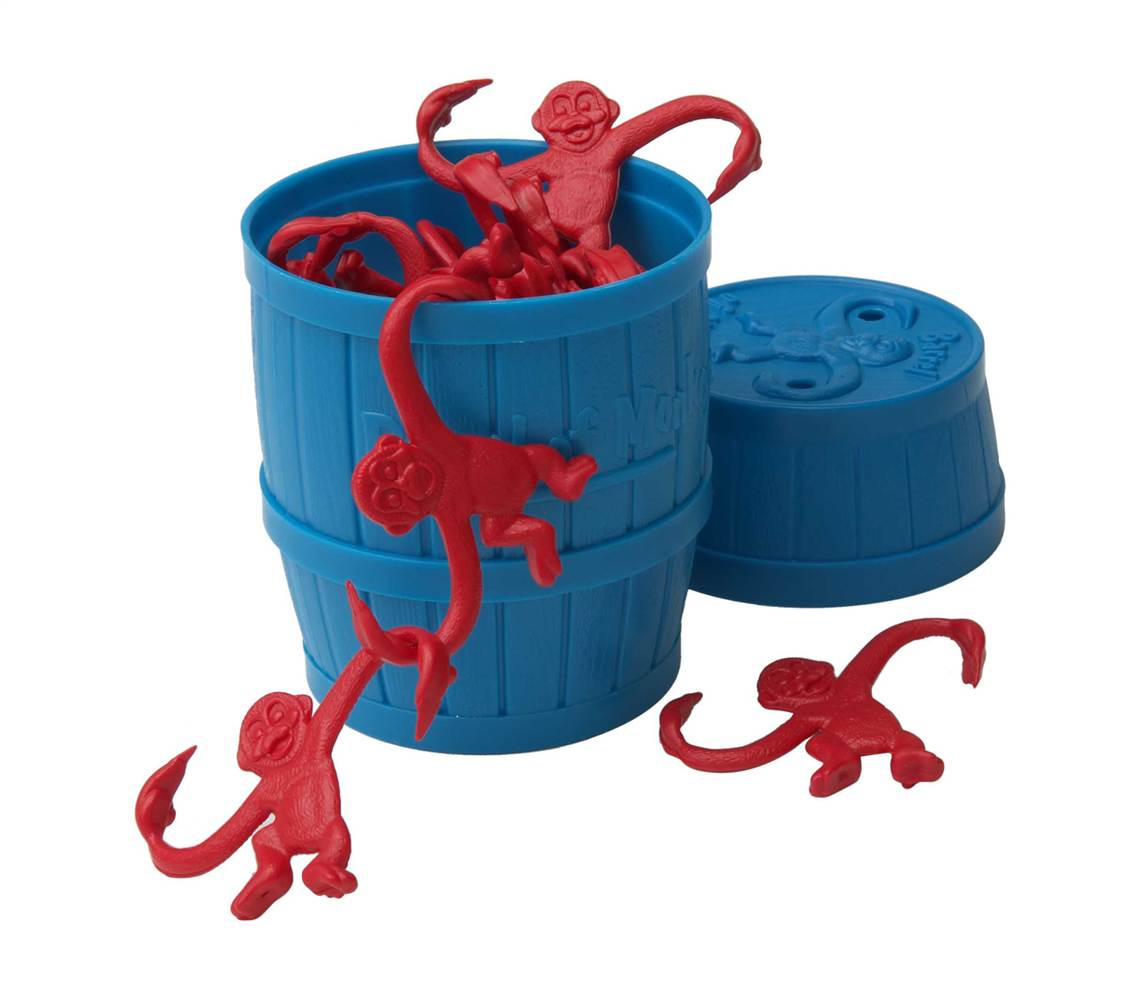
\includegraphics[width=12.1cm, height=9cm]{typescript/barrel-file/monkey-barrel}

\subsection{ Barrel File In Practice }
In the previous chapter we discussed doing something like the following:
\begin{lstlisting}
import {module} from '@ill/color-picker';
\end{lstlisting}

We are able to do this, because the nrwl nx layer on top Angular CLI, will
generate an index.tx file which will contain all imports. Anything that is
within the component, that should be exposed outside the lib, should be put
in the index.ts(barrel file).

\begin{lstlisting}[caption=index.ts]
export { IllColorPickerModule } from './src/ill-color-picker.module';
\end{lstlisting}

\subsection{ Enforcing Barrel File With Tslint }
In addition, Nrwl nx has a tslint add on called nx-enforce-module-bounderies.
\begin{lstlisting}
// tslint.json
"nx-enforce-module-boundaries": [
      true,
      {
        "allow": [],
        "depConstraints": [
          {
            "sourceTag": "*",
            "onlyDependOnLibsWithTags": [
              "*"
            ]
          }
        ]
      }
    ],
\end{lstlisting}

Adding true, will make the tslint complain whenever we are not using the barrel
import when accesing a lib file.

\maketitle{}
\section{ Using Angular CLI in an Nx Workspace }

Now that we have created an nx workspace, let's create our app. Run
\begin{verbatim}
  ng g app angularPixelIllustrator --routing
\end{verbatim}

This will create an app called angular-pixel-illustrator\footnote{that's right
angular cli will automatically convert camel case to dash case} with routing
capabilities using the Angular CLI \footnote{If you will recall, we discussed
the Angular CLI folder/file directory in the Angular CLI Chapter}.

We can now serve\footnote{I.e. run on a server for development reasons} our app,
by running:
\begin{verbatim}
  ng serve
\end{verbatim} \footnote{It's important to note, that ng serve will open up
angularPixelIllustrator by default. As we begin to add more apps, it will make
more sense to specify specific app being opened.}


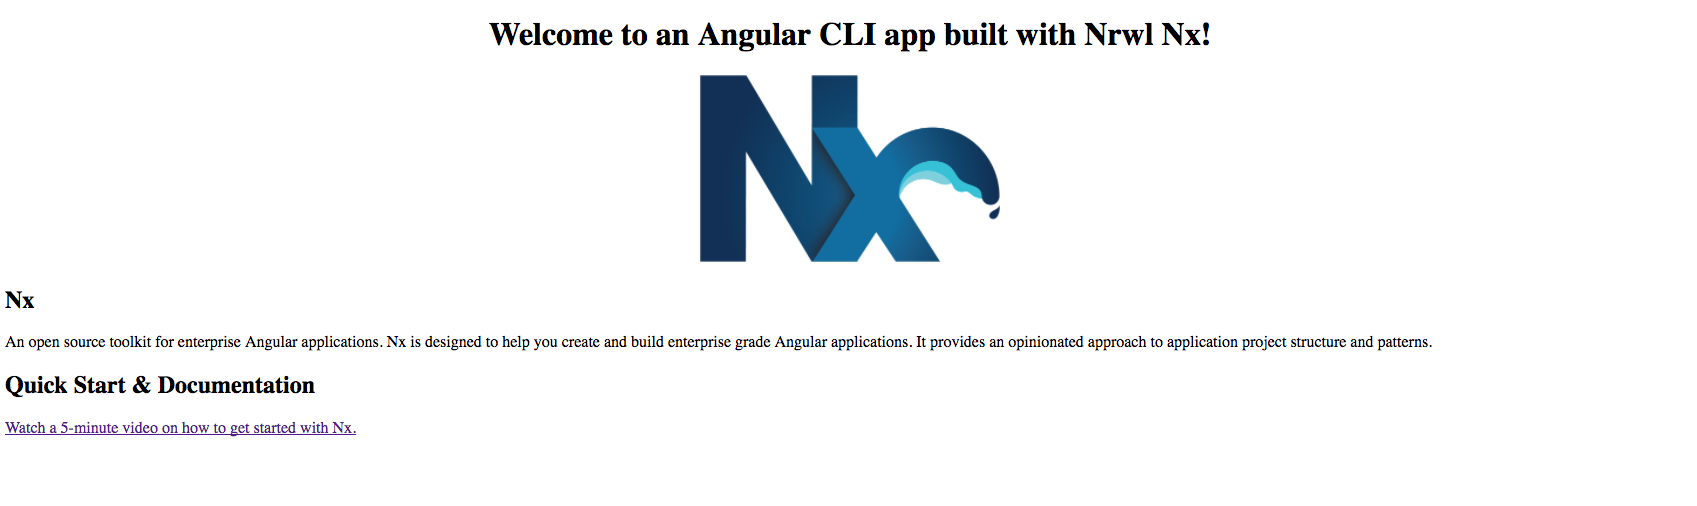
\includegraphics[width=13cm, height=9cm]{angular-cli-post-nx/angular_nx_initial_screen}

At this time, if you were to go to localhost:8080 you will see our app, is
ready to go.

Let's now create our first component. For our Pixel Illustrator, we want a form.
We will name the component chooseSize.

\subsection {Wait a Minute!}
Before we go ahead and create our component, we are going to want to tidy up
our folder architecture. The architecture we are introducing in this book is
heavily influenced by two projects. One, Nrwl, and by extension Nx. The other is
the example app, introduced in the ngrx/platform repo \footnote{It can be seen
here: https://github.com/ngrx/platform/tree/master/example-app}.

\subsubsection {Sidebar}
At the time of thiwriting there is one main area of conflict with regards to
ngrx/store v. Nx. Even though we have not experienced it yet, it makes sense to
talk about it before moving on from the cli/nx workspace chapters. Nx is very
opiniated with regards to it's folder structure. It believes everything should
be turned into it's own module, and all files related to that module should
be encapsulated inside of it. This includes (and if you are not familiar, do not
worry, we will get to it in later chaptes ) pipes, services, interfaces, guards,
and enums.

In the ngrx/example-app project, these will be split into separate folders, and
the appropriate file, will be put into that specific folder. I would imagine
that many on the ngrx/platform team agrees with nrwl/nx. I most certainly do,
and especially with state management, it makes sense for all others items to
be encapsulated into their appropiate folder. If it is something that should be
shared across app, then it should be put into it's own library. Something that
we will discuss moving forward.

\subsection {Phew, sidebar over, moving on}

The above being said, whenever we create a component, we are going to want to
encapsulate it, into a local module. That way we can add state, pipes, services,
you name it, and it will all be encapsulated in that component folder.

In order to create our module we run the following angular cli command:

\begin{verbatim}
  ng g module choose-size
\end{verbatim} \footnote{Once again we have the liberty with not having to
specify the app name}

Then, in order to create our component:
\begin{verbatim}
  ng g component choose-size
\end{verbatim}
The following five files have been created (using git diff --cached)
\begin{lstlisting}[breaklines]
new file:   apps/angular-pixel-illustrator/src/app/choose-size/choose-size.component.css
new file:   apps/angular-pixel-illustrator/src/app/choose-size/choose-size.component.html
new file:   apps/angular-pixel-illustrator/src/app/choose-size/choose-size.component.spec.ts
new file:   apps/angular-pixel-illustrator/src/app/choose-size/choose-size.component.ts
new file:   apps/angular-pixel-illustrator/src/app/choose-size/choose-size.module.ts
\end{lstlisting}


\section{ Format all the things }

In a Nrwl setting, we have a format npm script that is available to us by default.
It is called:

\begin{verbatim}
  nx format write
\end{verbatim}

This will call, a .prettier file that has been created by the nx workspace
command. Prettier is similar to to the CLI to the extent that there is a lot
that is happening behind the scenes. In short, it will automatically format files
for you, to it's liking. It's like a pro-active linter, that will format code
for you.

Two architectural talking points, with regards to prettier:
\begin{enumerate}
  \item You will have to format your tslint, so that it does not compete with prettier.
  \item You are going to want to hook up prettier with your IDE, so prettier
  can go to work without having to run it in your terminal.
\end{enumerate}

Note: We are going to have to create a way that we can update the prettier file
automatically.

\subsection{ How to add prettier to Webstorm }
As we mentioned in a previous chapter, Webstorm is our IDE of choice. VIM users
and Atom users, I completely respect your decision, and feel free to code in
that capacity. However, my experience working with large teams, is  that Webstorm
has a lot to offer outside of the box. For the non power user, it will offer
all of those benefits. Ok, great, the following is how to add prettier to Webstorm
with a screenshot!

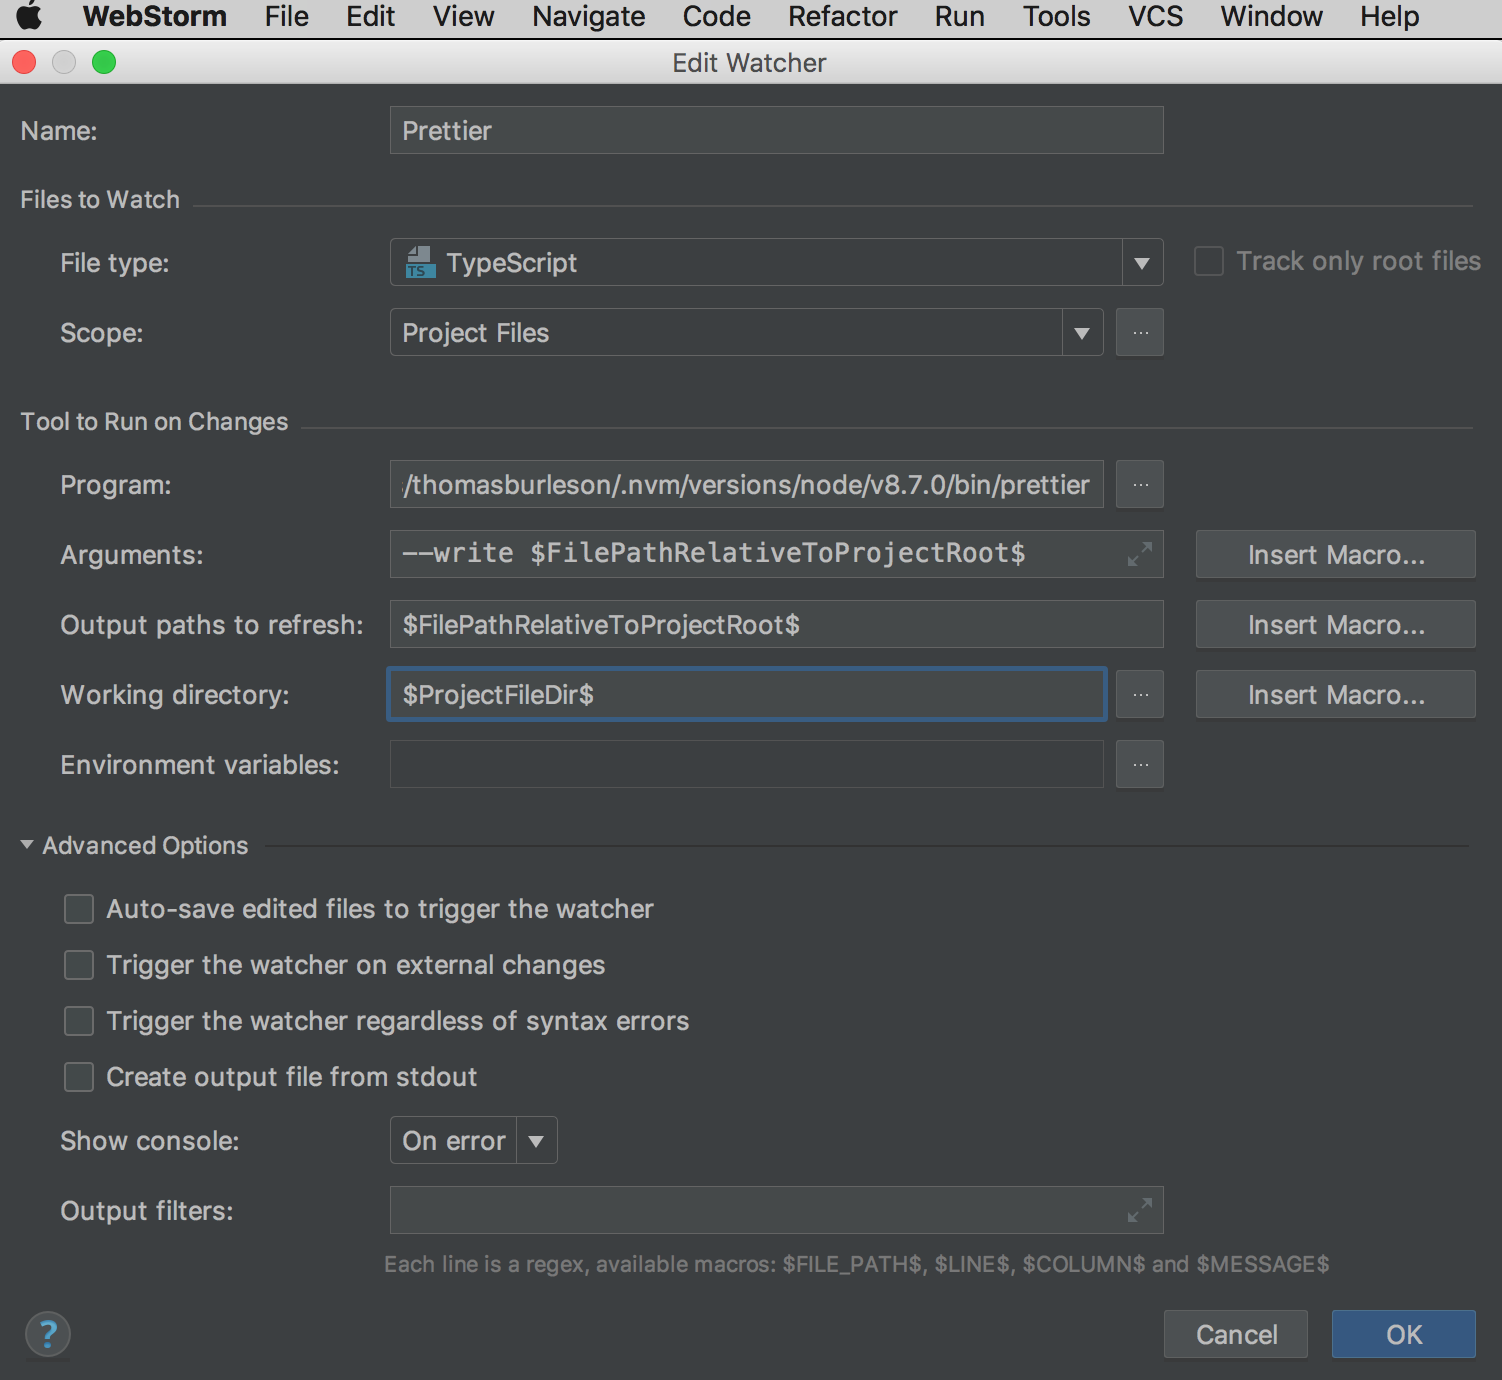
\includegraphics[scale=0.5]{format-all-the-things/prettier-file-watcher-webstorm}

\maketitle{}
\section{ Lint all the Things }

\subsection{ Lint all the Things }

Linting is incredibly important. Think of it this way. Someone's favorite food
item might be brocolli, another person's favorite food item, might be steak.
Now the two might work well together(on a number of levels, mmm hungry), but
forcing one person to adopt the other food item as their favorite, is unjust!

Ok, bad example, but the concept is the same. Things such as how many spaces per
indentation, double quotes vs. single quotes, trailing commas, empty interfaces,
these are all important points. To be honest, I've only found my peers arguing
on more minute points, such as double vs. single quotes, and how many spaces
per indentation. Therefore, linting allows:
\begin{enumerate}
  \item Agreement on code formatting rules.
  \item Automated way of keeping track of things that need to be changed.
  \item Self documentation through cli, on what needs to be changed.
\end{enumerate}

Another important point, is that we would ideally like a formatter, that
automatically formats these things for us. So, from an architectural perspective
when we are looking for a linter, we are also looking for a formatter to go along
with it.

\subsection{ What are we trying to lint? }
We are trying to lint HTML, SASS, and Typescipt. Angular CLI, offers Tslint out
of the box. 

\maketitle{}
\section{ Material Design }

I was debating writing this chapter. The reason primarily being, that depending
on the size of your company, you might up end writing your own design system. I
completely understand that, and it makes sense if you are a B2C
\footnote{Business to Consumer} enterprise.

However, I truly do not understand why a company using angular 5, or 6, would
not want to use material design. It is the most robust design framework that
exists within open source. In addition, the documentation for Angular components
is next to none. I personally have been in companies where they had a business
to business application and they decided not to use material design.

I really do not understand the reason for doing this. They could have saved
loads of resources not having to design and implement their own components. It
is out of the vast amount of use cases that I see Material Design being valuable,
that I have decided to go ahead and write about it.

\subsection{ Material Design - Talking to UX/UI }
This section right here, is perhaps why I like Material Design the most. Material
Design has documentation for how the UX should work. It also has an Angular
component library with demos, that I can show off to UX and show them, this is
how it works by default. It addition, theming for Material Design, is very easy.

Putting your own company specific spin on it, boils down to the following:
\begin{enumerate}
  \item Colors
  \item Font
  \item Spacing(Margin + Padding)
  \item Icons(not that this is anything particular)
  \item Buttons
\end{enumerate}

The above would be it for starters. As your designs go on, you will have components
that you will end up overridig.

\subsection{ Material Design - Create your own Confluence Doc }

It is important when working with UX/UI to document discrepencies. For
inspiraiton look at the \href{material design docs}{https://material.io/guidelines/components/sliders.html}.
The idea is to have a central place where UX can create Confluence doc
describing the differences they have made from DLS.

Engineers will generally have to be the one to begin the Confluence doc. From a
matter of ownership, engineering has a stronger discipline of documentation and
organization. Engineers should look to take ownership of the confluence doc.

\subsection{ Material Design - Use Invision }
It's interesting, because someone might not think of tooling as something which
is a part of engineering architecture. However, with regards to finding
discrepencies in DLS(Design Language System), Invision is integral. It will
make creating comments on particular components as something which will be fluid.

\subsection{ Material Design - Push Back }
The following will be worth alot of time for many different people within your
organization. Make sure that your component does not deviate from Material
Design. In addition, look into whether, or not it is pre-described for you to
go ahead, and create your own components. However, I can assure you designers,
product/business, and engineers will all be happy when you go with the default
components when possible. When building a product, unless it is beyond the MVP
go with what is available for you by default. 

\maketitle{}
\section{ Sass Error Reporting }

\subsection{ When to use Sass Error Reporting }
One should use Sass Error reporting if it is a core style. It is a core style if
it is used in more than one page, as a foundational piece of styling, non
unique to specific component.

\subsubsection{ What We Are Looking For With Using Sass Functions }
\begin{enumerate}
  \item No values other than these are used
  \item When a Pr comes our way, and we say to use the above, we have a function which is self documenting.
  \item Have a UI of sorts that also trains developers on how the internal of
  the DLS works, so that they should be aware if anything is wrong.
\end{enumerate}

\begin{lstlisting}
// Gutter variables, for padding + margin
// function to take in multiplier(8), which must emit of one of values within mc-space-amounts
@function mc-space-multiplier($n) {
  $ill-space-amounts: (0, 4, 8, 16, 24, 32, 40, 48, 56, 64);
  $ill-space-multiplier: 8;

  @if(index($mc-space-amounts, ($n * $mc-space-multiplier))) {
    @return #{$n * $mc-space-multiplier}px;
  }
  @else {
    @error "Must contain one of the following numbers: #{$mc-space-amounts}.";
  }
}
\end{lstlisting}

In this particular situation this helps, so that if the input passed to the
multiplier is not a number, it will complain. In addition, if the result is not
one of the multipliers, it will complain as well. So for instance, if the number
passed in, is 1.5, it will cause the function to error out, being that there is
no number 12, that is one of the ill space amounts.

\maketitle{}
\section{ Sass Unit Testing }

\subsection{ When Does Sass Unit Testing Make Sense? }
One of the concerns with any architecture, is over engineering. With regards to
unit testing Sass, to what extent should one unit test? Should it be for every
class, for every function, any core class used within a framework.

Being that we are going to be creating sass functions for our core theming, it
would make sense to unit test them as well. If they are going to be use in 10,
or more places per each app, then we would like to make sure, that they are
indeed working in the fashion that they should be.

\maketitle{}
\section{ Containers, Routing + Ngrx/router }

We now have a choose-size component, as well as a choose-size module.
The dynamics of our app, is that there will only be two parent pages. One will
be the choose-size page. The other will be the draw page. When a user goes to
the page for the first time, they will see the choose-size page. Therefore we
are going to add two routes in our app.

In our app.module.ts, we will use the existing RouterModule that has been
created by Nx, and include it in our RouterModule:

\begin{verbatim}
  // Inside imports add
   RouterModule.forRoot([
    {
      path: '',
      redirectTo: 'choose-size',
      pathMatch: 'full'
    },
    {
      path: 'choose-size',
      component: ChooseSizeComponent
    }
\end{verbatim}

\marginpar{git commit -m 'Add a routes to the RouterModule, for the choose-size page.'}

Now that we have redirected the default homepage to re-direct to the
choose-size page, let's try it out. Open up http://localhost:4200, and your page
should navigate to the choose-size page, with the text, "Choose Size Works",
towards the bottom of the page. 

\maketitle{}
\section{ Mobile First - Building a Progressive Web App }

When building a an enterprise application, think about building a Progressive
Web App. It will allow your web experience to be built to feel as if it is a
native app experience. Not only will it make it progressive, but it will make
your users feel as if they are a part of an experience that is all encompassing.
It will give them the overencompassing feeling that they are getting the best
experience possible \footnote{We will discuss moving the app over to a native
app soon using NativeScript.}. Swipe right on Progressive Web Apps \footnote{
That is a millenial joke, but also a darn good PWA pun.}

\maketitle{}
\section{ The Angular Service Worker - Implenting in App }

For those of you unaware, a service worker is a a script that runs in the web
browser that manages caching for an application. So let's say you are offline
and you are making a query in your app that you have already made before, then
the service workers will make it so that request can go through even without a
network request. In short, having a servie worker, can increase dependency on a
network, and will greatly increase the user experience.

\subsection{ Design Goals }
\begin{enumerate}
  \item Caching an application is like installing a native application.
  The application is cached as one unit, and all files update together.
  \item A running application continues to run with the same version of all
  files. It does not suddenly start receiving cached files from a newer version,
  which are likely incompatible.
  \item When users refresh the application, they see the latest fully cached
  version. New tabs load the latest cached code.
  \item Updates happen in the background, relatively quickly after changes are
  published. The previous version of the application is served until an update
  is installed and ready.
  \item The service worker conserves bandwidth when possible. Resources are only
  downloaded if they've changed.
\end{enumerate}

\subsection{ Manifest File }
To support the above design goals, Angular loads a manifest file. The manifest
describes the resources to cache and includes hashes of every file's contents
\footnote{taken from https://angular.io/guide/service-worker-intro}.

\subsection{ Using Angular CLI to Enable Service Workers }
In the chapter where we used ng new for the first time, we set it up with a flag
for service workers. [For practical purposes, if you did not use the flag for
creating service workers, use the link \href{https://angular.io/guide/service-worker-getting-started}{here}]
and follow through on the steps in the link. I believe in you! You can do this!

For academic purposes, here is what the service worker flag does:
\begin{enumerate}
  \item Adds the @angular/service-worker package
  \item Sets the Angular Cli serviceWorker option to true, so that it generates
  a manifest for every build
  \item Imports the ServiceWorkerModule, and registers the ngsw-worker.js file,
  which is the name of pre-build service worker script
  \item Creates a ngsw-config.json file, which configures defaults for service
  worker
\end{enumerate}

\subsection{ Simulating a Network Issue }
\begin{enumerate}
  \item Go to Chrome dev tools \footnote{write something here if person does not know how
  to do so}
  \item Go to the Network tab
  \item Check the Offline box
\end{enumerate}

If you service worker is properly being used, then the page will load normally,
as opposed to the page displaying, "There is no internet connection".

For further reading, by all means read through the documentation on Service
Workers, on the \href{https://angular.io/guide/service-worker-getting-started}{Angular.io}.
I agree, reading their documentation can be a bit bland at times, but it is
really thorough and more than get's the job done. Good job Angular documentation
person, or persons!

\maketitle{}
\section{ PWA Toolset - Physical Devices }

There is currently a formula with which devices to use. Latest regular sized
Iphone, and Iphone Plus. Latest Google Pixel non plus
\footnote{That's right, skip the Samsung.}. Latest Ipad + Ipad Mini. That
is it. These are mostly used as a way to see web in real time, as you are
developing your application.

Therefore, the reccomended Physical mobile devices are as follows:
\begin{enumerate}
  \item Iphone 8
  \item Iphone 8 Plus
  \item Google Pixel 2
  \item Ipad (2018)
  \item Ipad Mini 4
\end{enumerate}

\subsection{ Browser Dependencies }

The following is expected browser dependencies on Desktop:
\begin{enumerate}
  \item latest two Chrome releases
  \item latest two Firefox releases
  \item latest Safari
  \item latest Internet Explorer
  \item latest Internet Explorer
  \item latest Microsoft Edge
  \item Windows 10
  \item Windows 8
  \item macOS Sierra
\end{enumerate}

\subsection{ Testing Local Server on Physical Device }

Now that we have our physical devices that we would like to work on, let's set
up a way that we can test on these mobile devices. Ideally the following three
criteria should be solved:
\begin{enumerate}
  \item Url that remains the same for dev - to be used on mobile device
  \item When edit is made, it should update all mobile devides simultaneously
  \item Have all mobile devices in a central location, so that we can visibly
  see all changes that are being made
  \item synchronized interactions \footnote{Clicking on a button in one place
  change it in all other places.}
\end{enumerate}

\subsection{ Ghost Labs }

First, our winner for responsive testing is Ghost Labs. Ghost labs fulfills all
of the above criteria mentioned above. Going into short why we chose it over
all other contendors:
\begin{enumerate}
  \item Very easy to setup, and therefore removes overhead for initial setup
  \item There isn't anything required to install on different devices. It is
  simply a url that is used, and shared across device.
  \item Screenshots on remote mobile devices
  \item Ghostlab has a built in inspector for debugging
  \item One click workspace, in order to start up all devices once again.
  \item Presentation mode, allowing users to present web app.
\end{enumerate}

\subsubsection{ Setting up Ghost Labs }
First and foremost, buy the Ghost Lab Device Lab Selector. I can assure you, it
is an architectural decision. The whole point behind developing on a physical
mobile/tablet devices, is to improve developer workflow. So that any change that
happens, can be viewed immediatly. The device Lab selector serves that purpose.

Setting up ghost labs is as simple as running it in the mac application, and
being able to open on numerous devices. The following is a screenshot of what
you might see in you Ghostlab application:

\maketitle{}
\section{ PWA Toolset - Sauce Labs }

\subsection{ The Value of a Continuous Testing Cloud? }

As we have mentioned in the chapter for physical devices, we have quite a bit of
different platforms to work on. Ideally, we want an environment that we can set
up with E2E tests, as well as integration tests, and then run on all environments.
This is on top of the physical devices we already have. To clarify\footnote{i'm saying this a completely friendly way}

The idea of physical devices is as follow: to have a real time update of all
edits being done in your local environment, so that you can go ahead and have a
continuous local development environment.

The idea of a continuous testing cloud, is to be able to check that all devices
and browsers are being properly tested on. This will work strictly with one's
e2e tests.

\subsection{ Bring it to the Table - Why We Chose Sauce Labs }

At this point in time, there are really two main competitors, when it comes
down to continuous cloud computing:

\begin{enumerate}
  \item Sauce Labs
  \item BrowserStack
\end{enumerate}

Before we go into the above, endtest which is a fantastic up and comer, is
unfortunately a victom of it's own business model. While allowing users to
create a very simple version of tests, it also locks in users to it's platform.
There is no way of exporting these tests, and it makes it a very uncomfortable
place for many enterprises. This is precisely the type of application we are
trying to focus on, in this book, so we shall move on. \footnote{Even if I were
working on a small app, I would still not use endtest, for fear of scale}

\subsection{ Sauce Labs }

\includegraphics[scale=0.6]{pwa-toolset-sauce-labs/logo-sauce-labs}

Sauce Labs offers one thing particularly well, documentation.

\subsection{ Responsive Design }
\subsubsection{ Choosing a Framweork }
With regards to responsive design, there are a number of frameworks, one can
choose with regards to creating a web app. The following are quite popular:
\begin{enumerate}
  \item Foundation
  \item Bootstrap
  \item Semantic UI
\end{enumerate}

However, the above for a grid system tend to be overkill in my opinion.
Specifically, the direction many UI web app tend to head, is that it will only
be used on Desktop. For mobile and tablet, there will be a separate Android and
IOS app created. In addition, due to the nature of angulars component
architecture, the use of ready made components, containers for apps, are the
only thing which will actually have specific media queries.

It is strongly suggested that your own super lightweight grid is created, or
used. I think it is important to keep in mind that most grid systems can be
limited to 500 lines of code, or less. I personally prefer to use Skeleton
\footnote{http://getskeleton.com/\#grid}. However, I am in the process of
creating my own grid system using css-grid. (need to get back to this one).

Alternatively, creating our own grid system is also advantageous. That is the
direction that will make sense in any enterprise app. Generally, in any business
setting, from the business side they will decide on having a unique look and
feel. Setting up something for the app that works.


\chapter{ Creating a component }

For re-iteration purposes, the definition of a component is something consituting
of a larger whole. Ideally anything we can turn into a component in an Angular
environment, will help us. In addition, anything which we can re-use across the
app, is beneficial as well.

When creating components, Angular also makes use of modules. Once again, just to
re-iterate, a module is an independent unit, which is used to construct a larger
interallated construct.

Angular stays true to these two definitions. A component can only be declared by
one component. If it is used by two, or more Angular will complain, saying that it
is already used by another component. Which by definition only constitues a larger whole.
A module on the other hand, is simply an independent unit. If we ever want to use
our component with two components, we will need to include it as part of a module.

Therefore, it is reccomended as general good practice, whenever creating a
component (unless that particular component has children), to always create it
with a module. For other reasons as well, it is smart idea. We will get into
those later \footnote{If you can't wait, and want the full list now, go here to
find it}.

We have already created a component as needed for our router, but for redundancy
sake here are the steps again.

Also, because we will be using sass, let's make sure that our cli is using sass.
Open up the .angular-cli.json file, and change two areas. One:
\begin{verbatim}
  ng set defaults.styleExt scss
\end{verbatim}
This will make it, so that whenever we set up our components using the cli,
again it will be in sass. Second, change your existing styles.css file to
styles.scss.

Let's use the cli to create our first module called choose size.
\begin{verbatim}
  ng g module choose-size
  ng g component choose-size --exports
\end{verbatim}

(The file at this time is included in our app as a route. Let's remove the
default nrwl text from app, so that all we have is choose-size works.)

\section{Architecture time}

Before, we haphazardly created a component in order to introduce routers. Now
that we are going to work on our actual component, let's set aside to specific
items with regards to architecture.

Whenever we want to create a page for our application that will be used as a
route, it is a container. Something which is simply there to "contain" all of
our components. In the root of our app directory we are going to create a
container folder. \footnote{We are once again borrowing from the example-app
project in ngrx/store}

\begin{verbatim}
  mkdir containers
\end{verbatim}
We will also be needing to mention, that we will be
moving our choose-size directory to a newly created components folder.

cd into your containers folder, and create a choose-size-page module/component:
\begin{verbatim}
  ng g module choose-size-page
  ng g component choose-size-page
\end{verbatim}

In this choose-size-page component, we will be adding our choose-size component.

In order to do so, we will need to import the choose-size component in our Angular
app, and add it to our choose-size-page module like so:

\begin{lstlisting}[caption=Importing the choose-size module]
import { ChooseSizeModule } from  '../../components/choose-size/choose-size.module';

@NgModule({
  imports: [
    CommonModule,
    ChooseSizeModule
  ],
  declarations: [ChooseSizePageComponent]
})
\end{lstlisting}

In addition, we are going to want to make sure to add an exports key/value to
our choose-size module, so that by importing it, we have the respective
component available as well.

\begin{lstlisting}[caption=Adding choose-size component as export]
  @NgModule({
   imports: [CommonModule],
   declarations: [ChooseSizeComponent],
   exports: [ChooseSizeComponent]
  })
\end{lstlisting}

With the component module properly imported, we can now use the component in our
choose-size-page html file:
\begin{verbatim}
// choose-size-page.component.html
<app-choose-size></app-choose-size>
\end{verbatim}

\maketitle{}
\section{ Adding a Route to Our Container }

At this point, being that we did not initialize our app with routing
\footnote{So that we may learn as we develop}, we will need to add a routing
file to our app. In our app root, we will be adding an app.routing.module.ts
file.

It will look something like the following:
\begin{lstlisting}[caption=app.routing.module.ts file]
import { NgModule } from '@angular/core';
import { Routes, RouterModule } from '@angular/router';

import { ChooseSizePage } from './containers/choose-size-page/choose-size-page.component';

const routes: Routes = [
  {
    path: '',
    redirectTo: 'choose-size',
    pathMatch: 'full'
  },
  {
    path: 'choose-size',
    component:  ChooseSizePage
  }
];

@NgModule({
  imports: [RouterModule.forRoot(routes)],
  exports: [RouterModule]
})
export class AppRoutingModule { }
\end{lstlisting}

In it, we are redirecting the default path to go to the choose-size url. When
the url switches over to choose-size path, it will load the choose-size component.

We are also obviously going to import the AppRoutingModule in our app.module.ts
file:
\begin{lstlisting}[caption=app.module.ts file]
import { AppRoutingModule } from './app.routing.module';
@NgModule({
  imports: [
    //...
    AppRoutingModule,
    //..
\end{lstlisting}

We are also going to delete the competing:
\begin{lstlisting}[caption=app.module.ts file]
    RouterModule.forRoot(
      [
        {
          path: '',
          redirectTo: 'choose-size',
          pathMatch: 'full'
        },
        {
          path: 'choose-size',
          component: ChooseSizeComponent
        }
      ],
      { initialNavigation: 'enabled' }
    ),
\end{lstlisting}

That we had in our app.module.ts, to tidy up that app a bit.

Terrific, we now have our app by default re-routing to the choose-size url path
and loading the choose-size component. Let's move onto styling real quick next.


\chapter{ Styling a Component }

Styling a component, of course, is a very complex topic. With styling, as an
architect in an Angular setting, there are 4 things that you will have to keep
in mind:
\begin{enumerate}
  \item Pre-processor of choice(Scss, Less, PostCss, etc.)
  \section{ Pre-processor of choice }
  \item Design system
    \begin{enumerate}
      \item Material Design(Google)
      \item Fluent Design(Microsoft)
      \item Flat Design(Apple)
    \end{enumerate}
  \item Responsive design(even if you have a mobile/tablet app)
  \item Naming convention of CSS classes
\end{enumerate}

\section{ Pre-processor of choice }
For our preprocessor, we have chosen Sass. \footnote{Incude link for a
discussion of why that is}

\section{ Naming Convention }
For our naming convention, we will go with BEM. It is an extremely easy way
of setting a part a specific component from an html and css side of things. A
quick primer on BEM.
Block is a component. We will be using pascal casing for ours \footnote{Link to
airbnb style guide}
Element is a child of block. It uses an underscore. For instance:
\begin{verbatim}
<div class = 'ChooseSize__input'></div>
\end{verbatim}
M stands for modifier. A modifier is an element, which modifies an already
existing element.
\begin{verbatim}

\end{verbatim}


\section{ Design System }
In an Angular setting, the component library which seems to make most sense is
Material Components
\footnote{https://material.angular.io/components/categories}. For starters, it
is a complete design system. All component's design will be synonymous with
each other. In addition, it is in the process of creating a cdk, which makes
all of these components customizable. In addition, it is a really nice design,
and feels native to the way Angular works. I have used it versus other libraries
and I can really say the documentation is just fantastic. I have used it in more
complex settings(e.g. the data-table), and adding on new functionality has been
just a joy.

\section{ Adding Material Design to Our App }
First install Angular Material components and Angular Animations to our app.
\begin{verbatim}
  npm install --save @angular/material @angular/cdk
  npm install --save @angular/animations
\end{verbatim}

In addition, we will need to add default styling to our app, in order for
styling to be applied to our Angular Material component. Inside of our
styles.scss file, import the following.
\begin{lstlisting}
@import '~@angular/material/prebuilt-themes/deeppurple-amber.css';
\end{lstlisting}

\section{ Our first component }
In our app, we are going to create our first component. It is essentially a form
with three fields:
\begin{itemize}
  \item Columns
  \item Rows
  \item Pixel Size
\end{itemize}

In addition, there will be a button which will say, 'Create Grid'. We are also
going to wrap our component, with the <mat-card> component, add a width of
300, margin-top and center.

\subsection{ Notable Mention - @HostBinding }
In an angular app, many times, we will want to add a specific class to our
parent container. In our situation, we will be using BEM, and creating a
ChooseSize class. It will implement flex, and use justify content, in order to
center the <mat-card> component.

\begin{lstlisting}[caption=My Javascript Example]
import { Component, HostBinding, OnInit } from '@angular/core';

@Component({
  selector: 'app-choose-size',
  templateUrl: './choose-size.component.html',
  styleUrls: ['./choose-size.component.scss']
})
export class ChooseSizeComponent implements OnInit {
  @HostBinding('class') class = 'ChooseSize';
  constructor() {}

  ngOnInit() {}
}
\end{lstlisting}

By putting @HostBinding as a decorator \footnote{If not familiar with decorator
, it is a function that is run when particular class is called} within our app,
it causes the host class to have the ChooseSize class. We are then able to
target our host element our scss:
\begin{verbatim}
  :host.ChooseSize {
    display: flex;
    justify-content: center;
  }
\end{verbatim}

\section{ CSS Naming Convention }
In your modern day front end framework, such as Angular, generally, we do not
have to worry about clashing namespaces. \footnote{Historal footnote, the
turning point for me was with this article \href{https://glenmaddern.com/articles/css-modules}{here}}.
Many other issues with css at scale, have been solved as well, have been 
solved by the general ecosystem, scss included.

However, reccomended architecture is that one still use something like BEM. I
would like to argue for using BEM in an Angular setting:
\begin{enumerate}
  \item It allows for easy grep in code base, when inspecting element first
  within chrome.
  \item It documents the type of element that it is.
  \item It will give structure to html, without need of using pug, or some other
  html pre-processor.
  \item Ease's creation of classes for integration testing\footnote{Use a modifer
  for BEM}
\end{enumerate}

It should be noted, that within our app, the form has been made a particular
width, which will work on all screen sizes, without the need of adjusting width.
As we move along in our app, we will have the option to look into sitations
wherein we can use actual media queries.

\maketitle{}
\section{ State Management - @ngrx/store }

Ngrx/store is a layer on top of Redux. It is a state management tool that was
originally created, in order to solve two way binding performance issues within
Angular. \footnote{Need to further bring source for this one}. It then extended
as a way to bring redux natively to Angular, with the use of Observables.

Let's dive into integrating @ngrx/store into our app. \marginpar{This particular
component has been written in the fashion of TDD. However, another chapter
will be dedicated to TDD/BDD in order to specify this point specifically.}

\subsection{ Using nx ngrx to Generate State }

\subsubsection{ Create root state using nx ngrx }

First we are going to generate an empty root, for our StoreModule, as well as
our EffectsModule. Our StoreModule is responsible as a singular store object,
which will be holding all of store data. Our EffectsModule is a singular effects
object, which will be holding all of our effects. \footnote{We will discuss
effects in more detail later}

\begin{lstlisting}[language=Bash]
ng generate ngrx app --module=apps/angular-pixel-illustrator/src/app/app.module.ts --onlyEmptyRoot
\end{lstlisting}

\subsubsection{ Create component state using nx ngrx }

Next, we are going to create state for our choose-size component. This is done
with ease using nx ngrx \footnote{Trust me, I've been in situations where I
was not using a CLI. It is not good news}

Run the following command:
\begin{lstlisting}[language=Bash]
ng generate ngrx choose-size --module=apps/angular-pixel-illustrator/src/app/components/choose-size/choose-size.module.ts
\end{lstlisting}

This will generate the following files:
\begin{lstlisting}[language=Bash]
create apps/angular-pixel-illustrator/src/app/components/choose-size/+state/choose-size.actions.ts (684 bytes)
create apps/angular-pixel-illustrator/src/app/components/choose-size/+state/choose-size.reducer.ts (869 bytes)
create apps/angular-pixel-illustrator/src/app/components/choose-size/+state/choose-size.effects.ts (859 bytes)
create apps/angular-pixel-illustrator/src/app/components/choose-size/+state/choose-size.effects.spec.ts (1070 bytes)
create apps/angular-pixel-illustrator/src/app/components/choose-size/+state/choose-size.reducer.spec.ts (364 bytes)
\end{lstlisting}
And update the choose-size module,
\begin{lstlisting}[language=Bash]
update apps/angular-pixel-illustrator/src/app/components/choose-size/choose-size.module.ts
\end{lstlisting}

\subsubsection{ High level overview of nx ngrx }
So, you might be wondering, what do those files that nx ngrx generated actually
do? It will generate three files:
\begin{enumerate}
  \item Action
  \item Reducer
  \item Effect
\end{enumerate}

In addition, nx will add Typescript enums for the action types. It will also
add a respective spec file(unit testing) for the action + reducer file.

\colorbox{darkgray}{\color{white}{Unit testing Actions?}}

Unit testing an action, would simply say, when an action is dispatched, expect
it to be of a certain type. However, enums, as well as type checking, fulfills
that obligation. Therefore, if one is using Typescript along with enums, there
should be no reason for writing unit tests.

\subsubsection{ Installing Redux Dev Tools }
A state environment is incomplete without proper devtools. In particular, being
able to see an action fired, as well as the complete state of any given time,
is invaluable.

Google, "redux Devtools"\footnote{In a book format, in my humble opinion, more
valuable than a link}. It is offered by remotedev.io.

With the chooseSize ngrx nx command, we just made, you should see something like
this:

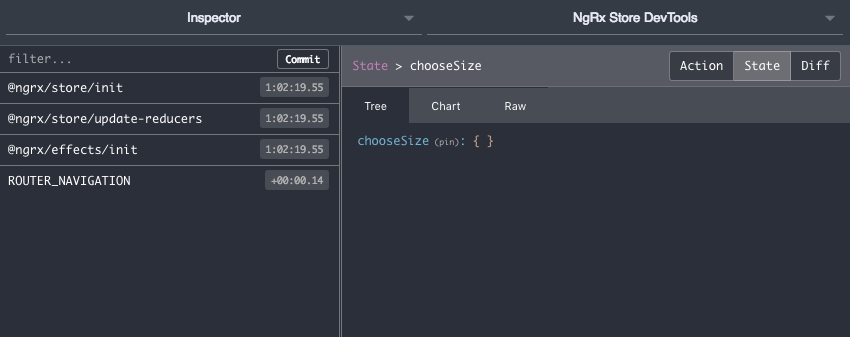
\includegraphics[width=13cm, height=9cm]{ngrx-store/redux-store}

\maketitle{}
\section{ Facade Pattern }

\subsection{ What is the Facade Pattern? }
The facade pattern is a classic. Anyone who has read the GoF book \footnote{
which if you haven't you should probably take a look.} knows that it is a
mainstay of computer science. Quoting from the GoF book:

\say{A facade is an object that provides a simplified interface to a larger body
 of code, such as a class library.}

\subsection{ A Look at your Typical Non Facade State Pattern  }
This pattern is particularly advantageous when it comes to ngrx actions. If I
may, let's imagine we have the following action:

\begin{lstlisting}
  // choose-size.actions.ts
export class LoadChooseSize implements Action {
  readonly type = ChooseSizeActionTypes.LoadChooseSize;
  constructor(public payload: any) {}
}
\end{lstlisting}

Now any time that we have to call an action we have to do two things:
\begin{enumerate}
  \item Have a store select within the component.
  \item Call a dispatch.
\end{enumerate}

\begin{lstlisting}
  chooseSize: Observable<any>;
  // choose-size.component.ts
  import { Store } from '@ngrx/store';
  constructor(private store: Store<any>) {
      this.chooseSize = store.select('chooseSize');
  //..
  merge(
    this.updateSize$.pipe(
      map((value: any) => new ChooseSizeUpdated(value))
    )
  ).subscribe(action => {
    store.dispatch(action);
  });
\end{lstlisting}

Obviously, this is quite a bit of overhead. Using the facade pattern let's see
if we can simplify this process.


\section{ Constants }

\subsection{ What is a Constant? }
In Javascript the idea of having a constant would be assigning a variable, to a
particular value. Whenever we would like that value, instead of typing out the
value, we would use the variable. At first, however, it might seem
counter-intuitive. Why use the constant value, if it is literally named the same
thing as the actual value?

\begin{lstlisting}[caption=Example of a Constant]
// Update last updated value to have latest payload data
const LAST_UPDATED = "LAST_UPDATED";
new updateValue(payload, LAST_UPDATED);
\end{lstlisting}

\subsection{ Benefits of a Constant }

\subsubsection { Creates a Table of Contents }
When one creates a series of constants in particular file for a certain
component, one can peruse through the constant file, being able to see all
actionable items in one. For instance, the following:

\begin{lstlisting}[caption=Example of a Constant]
// imagine these constants, are in a folder called ValueActionTypes
const UPDATE_VALUE = "UPDATE_VALUE";
const ADD_VALUE = "ADD_VALUE";
const DELETE_VALUE = "DELETE_VALUE";

//imagine the following code is in a new folder called valueActions
import * as types from "../ValueActionTypes";
import {BuyerValue} from './buyer-filter.interfaces';

export class UpdateValue implements Action {
  readonly type = UPDATE_VALUE;

  constructor(public payload?: BuyerValue, public keyName?) {};
}

export class AddValue implements Action {
  readonly type = ADD_VALUE;

  constructor(public payload?: BuyerValue, public keyName?) {};
}

export class DeleteValue implements Action {
  readonly type = DELETE_VALUE;

  constructor(public payload?: BuyerValue, public keyName?) {};
}
\end{lstlisting}

\subsubsection { Communicate to Maintainers }
If using a constant value, it signifies to future maintainers of your code, that
this is a value which is immutable. Further distinguishing intent of
application/snippet of code.

\subsubsection { Helps Secure Values }
When typing in a string for a particular constant value, particular diligence
must be applied in order to make sure it is type appropriately. Typing in the
one place, allows the developer to type in one place, and simply copy and paste
value, from a singular expected location(the const file) to 5 different places.

\maketitle{}
\section{ Enums as Constants }

When working with Typescript, which if you are using Angular, then you most
definitely are using Typescript \footnote{I look forward to working with
Reason sometime soon for typechecking, but I digress.}. Care must be taken to
look into all the nuances that Typescript can offer.

\subsection{ In a non Typescript Setting }

In order to define a constant in a non-Typescript setting, we use the const
declaration to define variables:

\begin{lstlisting}
  const UP = "UP";
  const DOWN = "DOWN";
  const LEFT = "LEFT";
  const RIGHT = "RIGHT";
\end{lstlisting}

\subsection{ Enums an Introduction }
Simply put, Enums allow us to define a set of named constants
\footnote{https://www.typescriptlang.org/docs/handbook/enums.html}.

\begin{lstlisting}
  enum PlaneActionTypes {
      Up = "[Plane] Up",
      Down = "[Plane] DOWN",
      Left = "[Plane] LEFT",
      Right = "[Plane] RIGHT",
  }
\end{lstlisting}

\subsection{ Benefit of Enums over Constants }
Enums allow us to organize a collection of related values. Think of them as
a class for values, wherein the value can only be a string , or number.

\subsection{ Current quirk of String Enums }
String Enums, as opposed to number Enums, have to be constant initialized
with a string literal. To clarify, you might want expect the following to work:

\begin{lstlisting}
  const prefix = '[Button]'
  enum Direction {
      Up = `${prefix} UP`,
      Down = `${prefix} DOWN`,
      Left = `${prefix} LEFT`,
      Right = `${prefix} RIGHT`,
  }
\end{lstlisting}

However, this does not work , because this is not a string literal, i.e. string
only.

\subsection{ Convention as a Result of Quirk }
As a result of quirk, we need a way of specifying that this action is happening
in relation to a specific object. Even though we do have a set using enums,
when identifying the string on it's own, from a state management (dev tool)
perspective, or console perspective, it will be beneficial to have the string
literal, be explicit on it's own. [Screenshot of a redux devtool would great].
Please reference above subsection, "Enums as an Introduction", for how this
translates to code in principle.

\subsection{ Side Note - Why No All Caps in Enums? }
A const in Javascript can actually be re-assigned to something else. For
instance:
\begin{lstlisting}
const PLANE = 'blackbird';
PLANE = 'thunderbird';
// barf
\end{lstlisting}
It is therefore a good convention when using a const, to put it in all caps,
when the value is not attend to be re-assigned such as:
\begin{lstlisting}
const PLANE = 'blackbird';
// woh, I was about to re-assign plane to thunderbird for some weird reason, but
// then I saw PLANE in all caps, so I didn't do it
\end{lstlisting}

However, this is not the convention with Enums, of course, because all enums
are never re-assigned. It is therefore not necesary to to write in all caps.

\maketitle{}
\section{ Integrating ngrx/store with Apollo Client }
In many architectures, it is most likely going to make sense that it is
microservice based. That is, your data will be served over a slew of different
apis. In which case the intent is that in a regular application, you will be
using GraphQL. It is reccomended that you use Apollo Client as well. We will
cover real quick, how to integrate GraphQL with Apollo Client.

\subsubsection{ What is GraphQL }
GraphQL is a backend data query language. It will allow you to use a query to
make a request, as opposed to having to supply, url, endpoint, and type of
request.

\subsubsection{ The Benefit of Apollo }
Apollo is a GraphQL client, used to help ease use of GraphQL http requests
within app. In particular:
\begin{enumerate}
  \item Allows the application developer to easily execute GraphQL queries, and
  configure transport-specific features like headers.
  \item Ensure that all GraphQL results currently being displayed in an app, are
   consistent with one another.
  \item Provide flexible ways to update the cache with results from the server
  when using mutations, pagination, subscriptions, and more.
\end{enumerate}

\subsubsection{ Dilemma When Using Apollo Client with @ngrx/store }
Apollo will create it’s own inMemoryCache, without dependency on Redux. However,
this creates two separate stores within the app when using @ngrx/store.
One for ngrx/store, and another for the Apollo client. It would be much easier,
obviously, if we had a singular cache/store, for the app.

\subsubsection{ Enter apollo-angular-cache-ngrx }
apollo-angular is a series of packages for the integration of the Apollo client
with Angular. apollo-angular-cache-ngrx is a package officially a part of one of
the apollo-angular packages. It solves this exact problem, and allows one to use
@ngrx/store as one’s Apollo Cache. (The following can be seen in the github
README.md for the apollo-angular-cache-ngrx repo, but going to put here for
convenience reasons).

\subsubsection{ Installation }
We will be wanting to install the entire apollo suite at this time.
\begin{lstlisting}
npm install apollo-angular apollo-angular-link-http apollo-link apollo-client graphql-tag graphql --save
\end{lstlisting}
As well as apollo-angular-cache-ngrx
\begin{lstlisting}
npm install apollo-angular-cache-ngrx —-save
\end{lstlisting}

\subsubsection{ Usage }
\begin{lstlisting}
import {StoreModule} from '@ngrx/store';
import {
  NgrxCacheModule,
  NgrxCache,
  apolloReducer,
} from 'apollo-angular-cache-ngrx';

@NgModule({
  imports: [
    StoreModule.forRoot({
      apollo: apolloReducer,
    }),
    NgrxCacheModule,
  ],
})
class AppModule {
  constructor(ngrxCache: NgrxCache) {
    const cache = ngrxCache.create({});
  }
}
\end{lstlisting}

If one were to now make an Apollo GraphQL query in your Typescript component,
your current ngrx/store will be populated with the appropriate Apollo data.
You will be able to subscribe to it as usual. For instance:
\begin{lstlisting}
  constructor(store: Store<any>, private apollo: Apollo) {
    this.store = store;
      apollo
        .query({
          query: gql`
            {
              users {
                status
                id
                name
              }
            }
          `
        })
        .subscribe((initialData: any) => {
          console.log(this.initialData);
        });
  }
\end{lstlisting}

At this time however, we are not using GraphQL within the above fashion.
Nonetheless, your average app, will be using this sort of architecture, and it
is very good to be aware of it, as well as how to use it.

\maketitle{}
\section{ Integrating a Component with @ngrx/store }

Another chapter has been dedicated solely to integrating a component
with @ngrx/store. This is because it is a cookie cutter process. Observables
are notoriously known, for abstracting events, and therefore allowing the same
code to be repeated time, and time again. The following is what can be expected
to be repeated time and time again in your application, after initially
generating files.

Just for redundancy sake, there are six steps, that go into setting up state
with any given component, that are handled by the nx ngrx cli:
\begin{enumerate}
  \item Store
  \item Action
  \item Store
  \item Reducer
  \item Initial State/Enums\footnote{In some other framework it might be constants}
  \item Effects
\end{enumerate}

All that is left, is for us to now to do three things component side:

\begin{enumerate}
  \item Set ups actions in view layer (i.e. HTML)
  \item Select store, so that it can be used in component
  \item Setup subject in component, so that it can be used with actions in view layer
  \item Set up subscribe in component(to transfer model to controller) \footnote{A subscriber is rarely setup in the smae component setting up the store to begin with}
\end{enumerate}

This is pretty standard, and this will be done in every standard application.
It is this simple, and will follow this formula, and yes, you should be in shock
in how seamless integrating state management technology is at this point,
because I am.

\subsubsection{ Re-iterating purpose of book }

I would just like to re-iterate, that the point of this book, is to go through
the architecture of the entire angular ecosystem. So that someone can read this
book and have the confidence that they are building their Angular app the proper
way, and that they do not have to look elsewhere. That being said, I will not be
going into the whole code base of what is happening. However, I would like to show
an example of along the lines of what will end up happening.

\subsubsection{ Creating a subject }

To re-iterate, what is a subject? It is both an observable and an observer?
\begin{enumerate}
  \item Observer — It has the next, error, and complete methods.
  \item Observable — It has all the Observable operators, and you can subscribe
  to him.
\end{enumerate}

Therefore, in an Angular setting, using @ngrx/store, subjects are our friends. It
allows us to have a singular event handler, to be used by all html event handlers
within component. In addition, it gives us a subscribe. The general pattern in
an Angular app will be as follows:
\begin{enumerate}
  \item Create subject in component
  \item Set up different namespace for unique actions in components
  \item Merge subjects into singular subscribe
  \item Which then emits payload per action
\end{enumerate}

\subsubsection{ Creating a Subject - Code Dive }

\maketitle{}
\section{ Unit Testing }

Unit testing has always been a hot topic. It's because it really isn't so well
understood amongst many software engineers. In addition, I know of many managers
who look as unit testing as icing on the cake. Good unit testing, is incredibly
difficult, and requires incredible amounts of due dilligence. Many books have
been written in this regard, and will not go into detail here.

However, what unit testing allows us to do, is assure the code we are
implementing is correct. Just as important, it sets testing in place, so that if
another developer changes something, such as the ordering of function
parameters, a class name, or a result of a function it will break. Unit testing
can also be set in place to make sure a certain function is called, when a
button is clicked, or in what order functions are correct. In can be set in
place as automatic self correcting code.

Unit testing, can also make our code self documenting. In addition, it can
give us the confidence moving forward knowing that this will work the way it
needs.

Unit testing really is a beast, and is really hard to manage. It's because it
isn't directly related to quality assurance, and can easily go under the radar,
as the app will go on without it. However, everytime that I have communicated
with management the bottom line. Research has been done on unit testing, and that
the application will be harder to manage long term, without it, they understand.
Bring the above point up to them, and hopefully you can have unit testing as a
part of your application.

At this point in our application, the only thing that we have created that
deserves to be unit tested, are the reducers. Let's go ahead and unit test those:

\begin{lstlisting}
describe('Functionality for the ChooseSizeUpdated reducer', () => {
  const chooseSizeData = {
    columns: 20,
    rows: 20,
    pixelSize: 20
  }
  it('should update the chooseSize store as is approprate', () => {
    const action: ChooseSizeUpdated = new ChooseSizeUpdated(chooseSizeData);
    const actual = chooseSizeReducer(initialState, action);
    expect(actual).toEqual(chooseSizeData);
  });
});
\end{lstlisting}

The above is an example of what a sample unit test for a reducer would look like
in the chooseSizeUpdated reducer.

Note: Add in section going over best conventions with regards to unit testing.

\maketitle{}
\subsection{ Unit Testing as a Discipline }

Unit testing is difficult, because it is a different discipline. In particular,
the above unit testing that we made, is a great example of poor unit testing.
We simply tested to make sure that all fields properly made their way over.

However, there are a number of considerations to keep in mind:
\begin{enumerate}
  \item What happens if we insert a string, instead of a number?
  \item Is there any limit on the number of rows, or columns?
  \item Should there be a limit on pixel size?
  \item Should there be a 1:1 ratio between rows and columns, or vice versa?
\end{enumerate}

\subsection{ The Irony of a Product Engineer }
One might think that the above requirments, are to be pro-offered by the Product
and to be tested by QA. However, at the end of the day, if these issues exist,
it will mean that the software you created will be lackluster. [This indeed
extends to other parts of the app, however, we are currently focusing on
unit testing]. Therefore, try to take ownership as an engineer. There are
different levels of intelligence, but amongst many other things, software
engineers are a truly analytical bunch.

\maketitle{}
\section{ TDD/BDD }

One of the tricky things with regards to E2E tests, is how it fits into a
TDD/BDD environment. Writing unit tests before we can see anything in our UI
already takes quite a bit of discipline. Adding in an E2E test to the workflow
seems like a bit much? Ok, so let's get into the thick of it. I think we'll all
have a good time!

\subsection{ What is TDD? }

\begin{enumerate}
  \item Start by writing a test
  \item Run the test and any other tests. At this point, your newly added test
   should fail. If it doesn’t fail here, it might not be testing the right
   thing and thus has a bug in it.
  \item Write the minimum amount of code required to make the test pass
  \item Run the tests to check the new test passes
  \item Optionally refactor your code
  \item Repeat from 1
\end{enumerate}

\subsection{ The Benefits of TDD? }
\begin{enumerate}
  \item Higher test coverage. \footnote{Emphasis is put on testing}
  \item Focus
    \begin{enumerate}
      \item Focus one part of issue one of a time.
      \item Allows one to realize when to stop coding.
    \end{enumerate}
  \item Interfaces
    \begin{enumerate}
      \item Allows you to think what is actually being baked into code more
      thoroughly. Allowing for interface to be written from the bottom
      up(behavior, implementation), instead of top down(implementation,
      behavior)
    \end{enumerate}
  \item Living Documentation. \footnote{Not to mention very verbose.}
  \item Enforces Pure Functions - Or re-usable code
    \begin{enumerate}
      \item As pure functions are easier to test, it will cause the developer
      to veer towards writing more pure functions.
      \item If pure functions are not an option, it will nonetheless cause the
      developer to veer towards re-usable code, and re-usable specs. \footnote{
      because this is the developer who is going to have to write tests time
      and time again.
      }
    \end{enumerate}
\end{enumerate}

\subsection{ What is BDD? }
Typically when testing a particular function at a later date, that function can
change it's implementation. For instance, the counter can start at 5, instead of
zero, breaking the expect statement of 1, when it is now 6. In BDD we focus on
the intended behavior, which is adding 1 to a particular value.

First things, first. Which comes first, unit test, or E2E tests? E2E tests will
end up going first, however, we will end up satisfying the unit tests first.

\begin{lstlisting}
// Non BDD
describe('Counter', () => {
  it('tick increases count to 1', () => {
    var counter = new Counter();

    counter.tick();

    expect(counter.count).toEqual(1);
  });
});

// BDD
describe('Counter', () => {
  it('should increase count by 1 after calling tick', () => {
    var counter = new Counter();
    var expectedCount = counter.count + 1;

    counter.tick();

    expect(counter.count).toEqual(expectedCount);
  });
});
\end{lstlisting}

\subsection{ The Benefit of BDD }
If at a later time the counter(as seen above), for instance, has to change
based on requirements(starting at 5, instead of 1), it will not affect the unit
test. That's it plain and simple, almost too simple, hmm... suspicious.

\subsection{ Convincing the Skeptic on TDD/BDD }
One of the equally most difficult things with unit testing, especially in a web
setting is coming across the various use cases, that will slow you down. Trying
to convince management, or whoever is in charge, that the amount of time that
you are spending on your unit tests, is going to validate the time taken towards
writing them. The following are some items that can be used towards convincing
the skeptic.
\begin{enumerate}
  \item Too simple to fail
    \begin{enumerate}
      \item If this is used regularly in our application, doesn't it then make
      sense to spend 5 minutes testing it?
    \end{enumerate}
  \item Too difficult to unit test
    \begin{enumerate}
      \item Good indication that it needs to be re-factored, proving point of
      benefit of unit testing.
    \end{enumerate}
  \item Too time consuming
    \begin{enumerate}
      \item App will produce more bugs.
      \item Lower quality code in regular app.
      \item Lack of confidence, perhaps bugs will be created under the radar.
      \item Lower design of system as a whole.
    \end{enumerate}
\end{enumerate}


\chapter{ Unit Testing TDD - First Princples Discovery }

Unit testing as a discipline is something which is very hard to write. Writing
a good unit test is as much as a discipline as writing good software. In
addition, if someone is following TDD standards, then knowing of all the unit
tests ahead of time can be very difficult. Leading many developers to leave the
TDD environment. If they do write unit tests, it will be towards the end. The
following is a great way, and as far as I am concerned the best way to discover
unit tests.

\section{ What is the First Princples Thinking? }
In Physics\footnote{Not a physicist, but I heard of this concept the first time
from Elon Musk. I am, however, a Talmudist, and in talmud we have a similar
concept called Pilpul}, there is a concept called, first principles thinking.
This means boiling down a priciple to it's essnetial truth and then building up
from there. With regards to Unit Testing, and specifically test driven
development, this principle will help to create fantastic unit tests.

\section{ First Princples Thinking - Rubber Ducking - An example }

\begin{lstlisting}
  Q: What would we like to get out of the choose size form?
  A: We would like to specify number of rows, number of columns, and pixel size.

  Q: Being that these are numbers, do we have any way of preventing
  the user from entering in any value other than an number?
  A: The input will only allow numbers.
  Q: Ok, do you see any value in setting up logic, so that if it is not a
  number, then it will throw an error?
  A: No, because there will never be a situation wherein they can not put in a
  number.
  Q: In that case, should we take a snapshot and make sure input fields are
  indeed of the type number. If not then it should error.

  Q: Now that we have established that these are always numbers, is there any
  limit on the size of this grid.
  A: Not really, I can see it as just being what the window size.
  Q: Hmm, I find that interesting, so you are saying that it can be any size.
  A: Yes for this iteration.
  Q: Okay, but it will be specific to window size.
  A: Yes.
  Q: Ok, so let's go ahead and create unit test, that it should have an
  error, that based on window size, if value is greater, it should automatically
  have it go to the height window size. In addition, there should be test that
  specifies as such.

  Q: Now that we have established that these we constrained window, is there any
  limit on the ratio between column size, and row size?
  A: No.
  Q: Is there any way that we can create a unit test, to just say that it
  passes, if there is a difference in ratio, between, then should not error out?
  A: Yes, need to figure this out though. Not sure how to do off hand.

  Q: Now that we have established that there are no constraints, what else is
  there for us to test. We have covered window size, ratio, input type, what
  about a max pixel Size?
  A: Hmm, why would we care about that?
  Q: Not sure, good point.

  Q: Hmm, that being said, should we only allow pixel size that is within the
  frame of the row and column size? For instance, let's say we have 20 rows, and
  20 columns, should the pixel size be something that perfectly divides into
  400?
  A: Not sure, it would be a lot of overhead at this point.
  Q: Almost feel like we should automatically control pixel size based on column
  and row size.
  A: Ok, out of scope, let's not.

  Q: Anything else?
  A: Not that I can think of.

  //End of Scene - dev takes a bow
\end{lstlisting}

To re-iterate in this book, we will not go into specifics of what is going on
at a particular time. However, these unit tests can be found in the Angular
Pixel Illustrator repo.

\maketitle{}
\section{ Unit Testing Component using Apollo }

Unit testing an app which has a DOM, is always a very difficult process. For
instance, one can be familiar with how a certain technology should be stubbed.
However, how one goes ahead and does so, is unique to that specific technology.
With regards to UI, frameworks currently tend to change very quickly. In
addition, thrre are many different frameworks, many of which use different
testing frameworks. It goes without saying, if I have a chance to learn
something and document it with regards to unit testing, it would be my honor to
do so.

In particular, with regards to the Angular Apollo Client. Until recently
(pre v1.1.0), using Apollo in an Angular App, was a very cumbersome ordeal.
In particular, there was no testing module. One would have to spin it up
themselves. However, now that we are dealing with v1.1.0, there is an official
testing suite set up.

\subsection { Re-visiting Component using Apollo }
First let's look at your standard Angular component generated by the Angular
CLI.

\begin{lstlisting}
import { Component, OnInit } from '@angular/core';

@Component({
  selector: 'ill-color-picker',
  templateUrl: './ill-color-picker.component.html',
  styleUrls: ['./ill-color-picker.component.scss']
})
export class IllColorPickerComponent implements OnInit {

  constructor() { }

  ngOnInit() {
  }

}
\end{lstlisting}

\subsection { Integrate Apollo with Component }

\begin{lstlisting}

+ import { Apollo } from 'apollo-angular';

+  ngOnInit() {
+    this.apollo
+      .query({
+        query: gql`
+          colors
+        `,
+      })
+      .subscribe((initialData: any) => {
+      });
+  }
\end{lstlisting}

\subsection { Unit testing Apollo }
First let's analyze what your generic Angular CLI generated spec will look like:
\begin{lstlisting}
import { async, ComponentFixture, TestBed } from '@angular/core/testing';

import { IllColorPickerComponent } from './ill-color-picker.component';

describe('IllColorPickerComponent', () => {
  let component: IllColorPickerComponent;
  let fixture: ComponentFixture<IllColorPickerComponent>;

  beforeEach(async(() => {
    TestBed.configureTestingModule({
      declarations: [ IllColorPickerComponent ]
    })
    .compileComponents();
  }));

  beforeEach(() => {
    fixture = TestBed.createComponent(IllColorPickerComponent);
    component = fixture.componentInstance;
    fixture.detectChanges();
  });

  it('should create', () => {
    expect(component).toBeTruthy();
  });
});

\end{lstlisting}

\subsection { Adding Apollo Testing Module }

\begin{lstlisting}
import {ApolloTestingModule} from 'apollo-angular/testing';
//..
+ ApolloTestingModule,
//..
\end{lstlisting}

The Apollo Testing Module will hijack the actual Apollo Module, and make it so
that there is no error in particular with regards to creating an apollo client.

\subsection { Hijacking the Component's GraphQL Request }
After we have imported our ApolloTestingModule within the app, we now need to
make it so that our GraphQL requests go straight to our fake backend request.
If we do not, of course, the colors GraphQL request will attempt to go the
default apollo link, making unit testing dependent on our GraphQL server.

\subsubsection { Initializing the ApolloTestingBackend }
\begin{lstlisting}
+ import {ApolloTestingBackend} from 'apollo-angular/testing/backend';

+ const mock = new ApolloTestingBackend();
\end{lstlisting}

ApolloTestingBackend works by keeping a list of all open operations.
As operations come in, they're added to the list. Users can assert that specific
operations were made and then flush them. In the end, a verify() method asserts
that no unexpected operations were made.
\footnote{This particular description can be found in: https://github.com/apollographql/apollo-angular/blob/master/packages/apollo-angular/testing/src/backend.ts}

\subsubsection { Initializing the Apollo Link }

\begin{lstlisting}
+ import {ApolloLink} from 'apollo-link';

+ const link = new ApolloLink(op => mock.handle(op));
\end{lstlisting}

An Apollo Link as the documentation mentions, is a function that takes an
operation and returns an observable. We are simply trying to repeat the process.
In particular for the execute function.

\subsubsection { Initializing the Operation }
\begin{lstlisting}
const operation = buildOperationForLink(query, {});
\end{lstlisting}

\subsubsection { Running the Execute Function }
\begin{lstlisting}
+ import {ApolloLink, execute} from 'apollo-link';

+ execute(link, operation as any).subscribe(result => (response = result));
\end{lstlisting}

\maketitle{}
\section{ E2E Testsing in a TDD/BDD Setting }

One of the tricky things with regards to E2E tests, is how it fits into a
TDD/BDD environment. Writing unit tests before we can see anything in our UI
already takes quite a bit of discipline. Adding in an E2E test to the workflow
seems like a bit much? Ok, so let's get into the thick of it. I think we'll all
have a good time!

\maketitle{}
\section{ Creating a Second Component }
Creating a second component within your app is a monumentous occasion. It lays
down the groundwork for how you are going to integrate numerous components
together within your app. Let's lay down at a high level what this means with
regards to a Mono Repo, in an enterprise Angular setting:

\begin{enumerate}
  \item Lib Folder
  \item Angular CLI Command
  \item Ngrx/nx ngrx considerations
  \item Routing Considerations
  \item Service Considerations
  \item Pipe Considerations
  \item Responsive Considerations
\end{enumerate}

\subsection{ Angular Pixel Illustrator - Example Use Case }
Let's take the above considerations into our app. The next component we are
going to create is a color picker. It will contain two sub components, a
background color picker, and a pixel color picker, re-used by a singular
component.

It will most definitely be going to into the lib folder. We will be using the
angular cli. We will be creating state, called color. With regards to a route,
we do want to create a generic route, that will switch out from the pixel grid
chooser, over to a a color picker view. We are also going to want a
consideration for mobile as this is a PWA. There aren't any pipes we will be
using.

\subsection{ Dissecting Business Requirements for Color Picker }
With regards to the color picker. There are three unique aspects of the business
logic:
\begin{enumerate}
  \item Color picker + Background Color Picker - Shared Logic
    \begin{enumerate}
      \item RGB
      \item HEX
      \item Convert RGB to HEX and vice versa
      \item Have color bar below pixel picker, change based on color value.
    \end{enumerate}
  \item Background Color picker
    \begin{enumerate}
      \item Change grid background, based on background color picker.
    \end{enumerate}
  \item Color picker
    \begin{enumerate}
      \item Change pixel color, based on pixel color picker.
    \end{enumerate}
\end{enumerate}

\subsection{ Creating a Second Component - Putting it all Together }
As we mentioned in the beginning in this chapter, this process is going to
be created each time we create a new component. Therefore, it would make sense
to sum up this process so we can repeat the process in every app. In addition,
for redundancy sake, we will go back to this checklist, and repeat the process.\\*

\begin{tabular}{@{} l *4c @{}}
\toprule
 \multicolumn{1}{c}{\color{red}Color Picker} & Need  & Do Not Need \\
\midrule
 @ngrx/store & \checkmark &            \\
 Route       & \checkmark &            \\
 Service     & \checkmark &            \\
 Pipe        &            & \checkmark \\
 Responsive  & \checkmark &            \\
\end{tabular}
\\*\\*
Regarding Business requirements:
\begin{verbatim}
  Scenario: When Using the Color Picker
    Given I enter Hex
    Given I enter RGB
    Then I should see state affected appropriately.
\end{verbatim}

You will notice for this particular component, the Then of our Aceptance
criteria, is oddly focusing on State. This is because due to the dynamics of our
system, this is what we are trying to focus on. However, if a product person
were to create it, one can expect it to be more hollistic, and to focus on
updating the grid as appropriate instead.

\maketitle{}
\section{ Pixel Grid Container }

\marginpar{Maintaining}
Now that we have created our Choose Size Form, let's go ahead and create our own
route for our presentation container.

\subsection{ Create Pixel Grid Container Component }
\begin{lstlisting}
cd containers
ng g module pixel-grid-page
ng g component pixel-grid-page --export
\end{lstlisting}

\subsection{ Import Pixel Grid Container Component }
In your app module, import the pixel-grid-page module. In the app routing
module, create a route for the pixel-grid-page.

\begin{lstlisting}
//app.module.ts
+ import { PixelGridPageModule } from './containers/pixel-grid-page/pixel-grid-page.module';

  ChooseSizePageModule,
+ PixelGridPageModule,
  NxModule.forRoot(),
\end{lstlisting}

\subsection{ Set up Router Link }
In any situation wherein a page has been created with routing, we are going
to need to create a routeLink, which will hook into the route which will be
created. In particular, in our app, we will be creating a routerLink on the
Create Pixel Grid button.

\begin{lstlisting}
//choose-size.module.ts
+ import { RouterModule } from '@angular/router';

+ RouterModule,
\end{lstlisting}

\begin{lstlisting}
//choose-size.component.html
+ <button routerLink="/pixel-grid"

+ RouterModule,
\end{lstlisting}

\maketitle{}
\section{ Flex Layout }

\marginpar{As we have just created the pixel-grid-page, now would be a great
time to implement Flex Layout}

\subsection{ Understanding the Issue With CSS Based Flexbox }
\begin{itemize}
  \item CSS specifity \footnote{CSS speicifity, is the means by which browsers
  decide which CSS property values are the most relevant to an element and,
  therefore, will be applied} issues rapidly become problemtic, and continue
  to be so.
  \item CSS footprint size becomes excessively large(>250k for flexbox CSS)
  whereas with JS, the module is loaded within every specific module
  \item Changes in layout direction required changes to child flexbox stylings
  \item No built in support for customized media query breakpoints \marginpar{
  need to look into further about what this means}

\end{itemize}

\subsection{ Why Use Flex Layout? }


\section{ Pixel Grid Container Layout }

Now that we have introduced Flex Layout and our designs call for three elements:
\begin{enumerate}
  \item Code Viewer
  \item Pixel Grid
  \item Color Picker
\end{enumerate}

\subsection{ Anticipate for Future Components }

We know that we will have three components that will be set up side by side.
On our main page component, which will contain all three, we will set the
following three fxLayout directives:
\begin{verbatim}
  fxLayout="row"
  fxLayout.xs="column"
  fxFlexFill
\end{verbatim}

The above is pretty straight forward. On screens not extra small, the layout
will be flex row. When the screen is extra small, the layout will be column.
With regards to fxFlexFill, it will populate the host element with the following:


\begin{tabular}{@{} l *4c @{}}
\toprule
 \multicolumn{1}{c}{Key} & Value \\
\midrule
 margin & 0         \\
 width  & 100\%     \\
 height & 100\%     \\
 min-width & 100\%  \\
 min-height & 100\% \\
\end{tabular}
\footnote{Taken from documentation here:
https://github.com/angular/flex-layout/wiki/fxFlexFill-API}

\subsection{ Adding FxLayout to Pixel Grid Page }

\subsubsection{ Add Flex Layout to App }
\begin{verbatim}
  npm i --save @angular/flex-layout
\end{verbatim}

\subsubsection{ Add Flex Layout to Pixel Grid Page Module }
\begin{lstlisting}
+import { FlexLayoutModule } from '@angular/flex-layout';

+    FlexLayoutModule,
\end{lstlisting}

\maketitle{}
\section{ Creating a Dumb Component }

\subsection {Outline}

\begin{enumerate}
  \item Create a UI dumb component in Lib folder
    \begin{enumerate}
      \item Use ClI to generate module
      \item Use ClI to generate component
    \end{enumerate}
  \item Import module into appropriate page
  \item Add component to page html
  \item Add proper styling to the illColorPicker
\end{enumerate}

\subsection {Create a UI Dumb Component in Lib Folder}
This is a dumb component, it should be created in the UI folder.
\footnote{Please reference the chapter discussing UI architecture for why
that is.}

\begin{lstlisting}
ng g lib color-picker --routing --directory="ui"
ng g component color-picker -a=color-picker --export
\end{lstlisting}

\subsection{ Add Color Picker to Pixel Grid Page Component }
Let's import our ill color picker into our Pixel Grid page.

\begin{lstlisting}
// pixel-grid-page.module.ts
+ import { IllColorPickerModule } from "@ill/ill-color-picker";
// in imports array
+ IllColorPickerModule
\end{lstlisting}

In addition, let's add the ill-color-picker component to our html.
\begin{lstlisting}
+ <ill-color-picker></ill-color-picker>
\end{lstlisting}

\subsection{ Add Styling Element to Create Basic  }
Let's add a basic width and height for out element.
\begin{lstlisting}
.IllColorPicker {
  display: flex;
  flex-direction: column;
  width: 200px;
  height: 100%;
}
\end{lstlisting}

\maketitle{}
\section{ Color Picker }

Let's go through the steps again, being that we are creating our second
component. Part of learning is not only discovery, but maintenance. As discussed
in the preface, whenever we have the chance to repeat steps we have discussed
once before, we will re-iterate them on a high level for memory sake.

\subsection{ Outline of what needs to be done }
\begin{enumerate}
  \item Create a UI dumb component for color picker in Lib folder
    \begin{enumerate}
      \item Should be generated in app folder in UI folder.
      \item Use ClI to generate module
      \item Use ClI to generate component
    \end{enumerate}
  \item Import module into pixel-grid page
  \item Add component to pixel-grid page html
  \item Add proper styling to the illColorPicker
\end{enumerate}

\subsection{ CLI - Creation of Module and Component with Routing }
First, let's create our component in the lib folder of our app.

\begin{lstlisting}
ng g lib color-picker --routing --directory="dealworks/ui"
ng g component color-picker -a=color-picker --export
\end{lstlisting}

\subsection{ Add Color Picker to Pixel Grid Page Component }
Let's import our ill color picker into our Pixel Grid page.

\begin{lstlisting}
// pixel-grid-page.module.ts
+ import { IllColorPickerModule } from ``@ill/ill-color-picker';
// in imports array
+ IllColorPickerModule
\end{lstlisting}

In addition, let's add the ill-color-picker component to our html.
\begin{lstlisting}
+ <ill-color-picker></ill-color-picker>
\end{lstlisting}

\subsection{ Add Styling Element to Create Basic  }
Let's add a basic width and height for out element.
\begin{lstlisting}
.IllColorPicker {
  display: flex;
  flex-direction: column;
  width: 200px;
  height: 100%;
}
\end{lstlisting}


\end{document}
